%% TeXworks instructions:
% !TeX root = ./report.tex
% !TEX encoding = UTF-8 Unicode
%% !TEX program = arara
%% !TEX TS-program = arara
% !TeX spellcheck = it-IT

% arara: pdflatex: { synctex: yes, action: batchmode, options: "-halt-on-error -file-line-error-style" }
% arara: pdflatex: { synctex: yes, action: nonstopmode, options: "-halt-on-error -file-line-error-style" }

%% Generate a report.xmpdata file with title and authors for PDF/A-compliant format %%
\begin{filecontents*}{\jobname.xmpdata}
    \Title{Maraph1-mp Project Report}
    \Author{Nicholas Brasini\sep Gjulio Jakova\sep Federico Naldini\sep Jacopo Riciputi}
\end{filecontents*}

\documentclass[%
    a4paper,            % specifica il formato A4 (default: letter)
    10pt,               % specifica la dimensione del carattere a 10
    oneside,            % serve per impaginare per stampa solo fronte
    notitlepage         % mette il titolo in una pagina separata (solo per article)
]{article}

\usepackage{a4wide}             % consente di avere più spazio nell'A4

%% ORDINE IMPORTANTE INIZIO %%%%%%%%%%%%
\usepackage[T1]{fontenc}        % serve per impostare la codifica di output del font
\usepackage{textcomp}           % serve per fornire supporto ai Text Companion fonts
\usepackage[utf8]{inputenc}     % serve per impostare la codifica di input del font
\usepackage[
    english,            % utilizza l'inglese come lingua secondaria
    italian             % utilizza l'italiano come lingua primaria
]{babel}                        % serve per scrivere Indice, Capitolo, etc in Italiano

\usepackage{lmodern}            % carica una variante Latin Modern prodotto dal GUST
%% ORDINE IMPORTANTE FINE %%%%%%%%%%%%%%

\usepackage{indentfirst}        % serve per avere l'indentazione nel primo paragrafo
\usepackage{setspace}           % serve a fornire comandi di interlinea standard
\usepackage{xcolor}             % serve per la gestione dei colori nel testo
\usepackage{graphicx}           % serve per includere immagini e grafici

\graphicspath{{./images/}}

\usepackage[%
    strict,             % rende tutti gli warning degli errori
    autostyle,          % imposta lo stile in base al linguaggio specificato in babel
    english=american,   % imposta lo stile per l'inglese
    italian=guillemets  % imposta lo stile per l'italiano
]{csquotes}                     % serve a impostare lo stile delle virgolette

\usepackage{multirow}           % aggiunge la possibilità di raggruppare celle su più righe nelle tabelle

\onehalfspacing%                % Imposta interlinea a 1,5 ed equivale a \linespread{1,5}

\setcounter{secnumdepth}{4}     % Numera fino alla sottosezione nel corpo del testo
\setcounter{tocdepth}{4}        % Numera fino alla sotto-sottosezione nell'indice

\usepackage[%
    depth=3,            % equivale a bookmarksdepth di hyperref
    open=false,         % equivale a bookmarksopen di hyperref
    numbered=true       % equivale a bookmarksnumbered di hyperref
]{bookmark}                     % Gestisce i segnalibri meglio di hyperref
\usepackage{hyperref}           % Gestisce tutte le cose ipertestuali del pdf
\hypersetup{%
    pdfpagemode={UseNone},
    hidelinks,          % nasconde i collegamenti (non vengono quadrettati)
    hypertexnames=false,
    linktoc=all,        % inserisce i link nell'indice
    unicode=true,       % only Latin characters in Acrobat’s bookmarks
    pdftoolbar=false,   % show Acrobat’s toolbar?
    pdfmenubar=false,   % show Acrobat’s menu?
    plainpages=false,
    breaklinks,
    pdfstartview={Fit},
    pdfauthor={Nicholas Brasini, Gjulio Jakova, Federico Naldini, Jacopo Riciputi},
    pdfcreator={Nicholas Brasini, Gjulio Jakova, Federico Naldini, Jacopo Riciputi},
    pdftitle={Maraph1-mp Project Report},
    pdflang={it}
}
\usepackage[utf8]{inputenc} % serve per avere l'indice di tutti i capitoli all'inizio 

\usepackage[section]{placeins} % serve per posizionare le immagini esattamente dove le inseriamo

%\usepackage[a-1b]{pdfx}
\usepackage[%
    english,italian,    % definizione delle lingue da usare
    nameinlink          % inserisce i link nei riferimenti
]{cleveref}                     % permette di usare riferimenti migliori dei \ref e dei varioref

\usepackage{fancyhdr} % serve per visualizzare nel top della pagina il capitolo corrente e la sezione corrente
\pagestyle{fancy}

\title{\LARGE{\textbf{Maraph1-mp Project Report}}}

\author{%
    Nicholas~Brasini\\%
    Gjulio~Jakova\\%
    Federico~Naldini\\%
    Jacopo~Riciputi
}

\date{%
    \small{Paradigmi di Programmazione e Sviluppo}\\%
    \small{Anni accademici 2017--2018 e 2018--2019}
}


\begin{document}
	
    \maketitle
    \clearpage
	\tableofcontents
	\clearpage
	
    \section*{\Huge {Capitolo 1}\label{chapter1}}
      \section{Processo di sviluppo}\label{sec:process}
        \subsection {Metodologia di sviluppo}\label{subsec:metodology}
        Il primo passaggio per poter iniziare a lavorare al progetto d'esame per la materia Paradigmi di Programmazione e Sviluppo è stato quello di selezionare la modalità con cui procedere per sviluppare il progetto stesso. Abbiamo dunque scelto di utilizzare una forma semplificata di metodologia \textbf{Agile Scrum}. Nella versione da noi adottata i quattro membri sono tutti allo stesso livello: abbiamo infatti scelto di rinunciare alla figura dello \textbf{Scrum Manager} dal momento in cui siamo partiti tutti dalla stessa base di conoscenze relative a questa metodologia e abbiamo preferito non sovraccaricare di lavoro un solo membro del team, responsabilizzando ognuno di noi a lavorare al meglio delle proprie possibilità per semplificare il lavoro degli altri. Come abbiamo studiato nel corso, ci siamo resi conto di dover utilizzare un supporto tecnologico per poter gestire efficientemente i singoli sprint. A questo proposito abbiamo scelto \textbf{Trello}, un'applicazione per gestire progetti di qualunque tipologia che ci ha permesso di poter controllare il progresso dei diversi compiti assegnati ad ogni membro del team (una panoramica più specifica dell'utilizzo di questo strumento verrà presentata all'interno del Capitolo 5). Nel corso della prima riunione effettuata dopo aver ricevuto l'approvazione della proposta di progetto, abbiamo stabilito che gli sprint avrebbero avuto cadenza settimanale (nella fattispecie ogni giovedì pomeriggio) e che sarebbero stati cinque (numero medio consigliato per chi adotta la metodologia Agile in un contesto di questo tipo). In generale, nel corso di ogni riunione settimanale, abbiamo valutato quanto fatto nel corso della settimana trascorsa ma soprattutto abbiamo stabilito quali \textit{item} (elementi) del \textit{product backlog} sviluppare in vista dell'incontro della settimana successiva, dopo aver fatto una stima del costo di ciascun item. L'assegnamento degli item è stato fatto di comune accordo, secondo le richieste e le capacità di ciascuno in maniera tale da agevolare chi avesse già conoscenze pregresse per esempio in ambito di database o di comunicazione ad attori. Abbiamo poi previsto la possibilità che alcuni membri del team potessero contattarsi e coordinarsi individualmente, come ad esempio è successo nel caso dell'integrazione della versione core, senza bisogno di dover interpellare tutto il team. Oltre all'incontro settimanale, abbiamo deciso di effettuare \textbf{Daily Scrum} della durata di una decina di minuti, che ci hanno consentito di calarci fino in fondo nella parte di sviluppo Agile ma soprattutto di poter gestire meglio tutti gli item sui quali stavamo lavorando. Così facendo, ci siamo accorti che in alcune situazioni gli item definiti in precedenza avrebbero avuto bisogno di essere ritoccati: il singolo membro del team aveva dunque la possibilità di informare gli altri giornalmente su eventuali modifiche apportate ad uno o più item su cui stava lavorando. Questa scelta si è rivelata essere particolarmente fruttuosa, poiché ogni membro del team si è sentito responsabilizzato e ha potuto effettuare cambiamenti in corso d'opera senza per questo inficiare il lavoro dei propri colleghi. In generale la scelta di adottare questa metodologia di sviluppo ha soddisfatto tutti i componenti del team, che si sono resi conto di quanto il raggiungere settimanalmente un risultato abbia portato un maggior entusiasmo e vitalità per poter affrontare gli incarichi successivi. Oltre a questa motivazione, è importante sottolineare come, in ottica futura, la possibilità di presentare ad un ipotetico cliente il prodotto che viene realizzato di settimana in settimana possa stimolarlo e renderlo più partecipe alla vita del progetto, con i risultati che tenderanno ad essere migliori rispetto ad un approccio di tipo classico.
        
        
        \subsection {Strumenti adottati}\label{subsec:tools}
        Dopo aver optato per la metodologia di sviluppo descritta nel paragrafo precedente, ci siamo trovati di fronte alla scelta dello strumento di \textit{versioning}. Per il nostro progetto abbiamo deciso di utilizzare \textbf{Git} e ci siamo serviti di \textbf{GitHub} per avere un \textit{repository} remoto gratuito. Contrariamente a quanto fatto per progetti precedenti, ci siamo avvicinati all'inesplorato (per noi) mondo di \textbf{GitFlow}, che si è rivelata essere una risorsa preziosissima per il raggiungimento dell'obiettivo finale. Per evitare di sviluppare su un branch comune, abbiamo dunque deciso di avvalerci dell'utilizzo di GitFlow, che ha permesso ad ogni membro del team di aprire, ogni volta che se ne fosse presentata l'occasione, una nuova feature sulla quale programmare in totale libertà senza paura di "rovinare" il lavoro degli altri colleghi. Abbiamo dunque deciso di utilizzare tre tipologie principali di branch:
\begin{itemize}
\item \texttt{master}. In questo branch abbiamo pubblicato solamente le versioni finali del progetto. Con la versione 1.0 abbiamo contrassegnato il termine della versione \textit{core}, mentre con la 2.0 il termine di quella distribuita.
\item \texttt{develop}. Questo branch ha rappresentato il punto di partenza di ogni nuova feature e, al termine di quest'ultima, il canale su cui riversare tutto il lavoro prodotto. 
\item  \texttt{generic feature}. Quest'ultima tipologia in realtà caratterizza tutte le feature create dai membri del team per lavorare ad uno specifico item. In generale abbiamo cercato di rispettare il \textit{topic} della feature andando ad effettuare solamente le modifiche all'item preso in considerazione.
\end{itemize}
Per effettuare invece il building del progetto abbiamo deciso di utilizzare \textbf{Gradle}, uno dei principali sistemi di automatizzazione delle build. Grazie ad esso abbiamo semplificato anche l'esecuzione dei test, la gestione delle dipendenze e la creazione dei jar da consegnare alla scadenza del progetto. Per poter sviluppare un progetto solido è necessario utilizzare sistemi di testing che ne verifichino l'integrità dopo ogni modifica. Lo strumento che abbiamo scelto di utilizzare a tal proposito è \textbf{TravisCI} che abbiamo successivamente collegato al repository creato su \textbf{GitHub} dal momento che permette di poter usufruire, in maniera gratuita, di funzionalità di \textit{Continous Integration}. 
        
        
        
        
        \clearpage
        
    \section*{\Huge {\textbf Capitolo 2}\label{chapter2}}
    \section{Requisiti}\label{sec:requirements}
    Il progetto d'esame \textbf{Maraph1-mp} si è posto come obiettivo quello di creare una versione distribuita e multi-giocatore del classico gioco di carte romagnolo \textbf{"Marafone"}, conosciuto anche come \textit{Marafona}, \textit{Maraffa} o \textit{Beccaccino} a seconda della città di appartenenza. Il gioco consiste in una schermata 2D all'interno della quale sono visibili solamente le carte del player che stiamo impersonando, mentre quelle del compagno (posizionato di fronte a noi) e quelle dei due avversari (posizionati uno a destra ed uno a sinistra rispetto alla nostra posizione) risultano essere coperte. Il gioco procede fino a quando una delle due squadrex risulta essere la vincitrice: a quel punto la schermata di gioco viene chiusa e si torna alla finestra di default, diversa sulla base del fatto che un player si sia registrato e loggato oppure no.
    
         \subsection {Requisiti utente}\label{subsec:requirements:business}
         Per questo progetto l'importanza dell'utente è centrale. Esso interagirà infatti con altri utenti giocando insieme a loro a \textit{Marafone}. 
         \begin{itemize}
         \item L'utente potrà scegliere se registrarsi al sistema oppure no
	 \item Se l'utente si registra:
	 
	 \begin{itemize}
	 \item Possibilità di interagire con i propri amici attraverso una schermata Social.
	 \item Possibilità di aggiungere al proprio elenco di amici i giocatori che sono online.
	 \item Possibilità di invitare i propri amici per una partita in qualità di compagno o di avversario.
	 \item Possibilità di giocare una partita in modalità competitiva, con aumento/diminuzione del proprio punteggio sulla base dell'esito della partita stessa. 
	 \item Possibilità di guardare i replay delle partite giocate da se stesso e da tutti gli altri utenti.
	 \item Possibilità di accedere come spettatore alle gare attualmente in corso.
	\end {itemize}
	
	\item Se l'utente non si registra:
	
	\begin{itemize}
	\item Non potrà accedere a tutte le funzionalità Social.
	\item Unica modalità di gioco quella non competitiva, ovvero senza punteggio.
	\item Possibilità di accedere come spettatore alle gare attualmente in corso.
	\end {itemize}
	
	\end {itemize}
         \clearpage
             \subsection {Requisiti funzionali}\label{subsec:requirements:functional}
             Dall'analisi del caso di studio sono state individuate le seguenti parti del progetto:
             
             \begin {itemize}
             \item Gioco
             \item Servizio di Autenticazione
             \item Servizio delle Stanze di gioco
             \item Servizio di Spettatore
             \item Servizio di Replay
             \item Funzioni Social
             \item Interfaccia Utente
             \end {itemize}
             
            \subsubsection[Gioco]{\large {Regole del gioco}\label{subsub:requirements:game}}
            Prima di iniziare a parlare dei requisiti del gioco, è bene analizzare le regole che caratterizzano una partita. 
            
            \begin {itemize}
            \item La partita inizia nel momento in cui sono presenti quattro giocatori all'interno della stessa lobby.
            \item Ad ogni giocatore saranno distribuite, in maniera totalmente casuale, 10 carte, per un totale di 40 carte in gioco.
            \item Le carte si suddividono in quattro semi: \textbf{Bastoni}, \textbf{Spade}, \textbf{Denara} e \textbf{Coppe}.
            \item Il gioco è suddiviso in set e turni. Un set termina quando tutti i giocatori hanno giocato una carta, mentre il turno finisce nel momento in cui tutte e dieci le carte di ogni giocatore sono state giocate.
             \item Fondamentale il concetto della briscola: si tratta di un seme che viene stabilito all'inizio del turno e supera il valore degli altri semi, sebbene sulla carta valgano di più.
              \item Nel corso del turno iniziale, viene scelta la briscola dal giocatore che troverà, all'interno delle proprie carte, il 4 di \textbf{Denara}. Dai turni successivi la briscola verrà scelta in senso antiorario, quindi dal giocatore alla sinistra dell'ultimo giocatore che ha scelto la briscola.
            \item Ad ogni turno vengono messi in palio 11 punti, 14 in caso di \textit{Maraffa} (ovvero la presenza dell'Asso, del Due e del Tre dello stesse seme nella mano del giocatore che deve selezionare la briscola).
             \item Ai giocatori non è concesso parlare se non attraverso tre possibili comandi: \textbf{Busso} (significa che il compagno deve giocare la carta più alta del seme giocato per provare a vincere il set e in quello successivo giocare nuovamente una carta dello stesso seme), \textbf{Volo} (significa che il giocatore non ha più carte del seme appena giocato) e \textbf{Striscio} (significa che il giocatore ha rimasto un'altra carta del seme appena giocato).
            \item I comandi possono essere comunicati solamente dal primo giocatore che inizia uno specifico set.
            \item Nel momento in cui viene giocata una carta di un certo seme, gli altri giocatori saranno costretti a rispondere con una carta dello stesso seme. Nel caso in cui il giocatore avesse terminato le carte di quello specifico seme, la scelta della carta da giocare sarà libera.
            \item L'azione del \textit{tagliare} prevede il fatto che venga giocata una briscola sopra ad una carta di un altro seme: questo nella maggior parte dei casi permette a chi ha tagliato di vincere il set. 
            \item La carta più potente, a parità di seme, è il \textbf{Tre}, seguito dal \textbf{Due} e dall'\textbf{Asso}. In cascata ci sono poi il \textbf{Re}, il \textbf{Cavallo} e il \textbf{Fante}, che sono considerate \textit{figure}, mentre le carte rimanenti sono considerate \textit {scartini}.
            \item Tutte le figure valgono 1/3 di punto, ad eccezione dell'Asso che vale 1 punto. Gli scartini valgono 0 punti.
            \item La partita finisce quando una squadra raggiunge i 41 punti o, in caso di parità a quota 41, quando una delle due squadre supera l'altra al termine del turno successivo. 
            \end {itemize}

            \subsubsection[Autenticazione]{\large {Servizio di Autenticazione}\label{subsub:requirements:auth}}
            Il servizio di Autenticazione dovrà:
            
            \begin {itemize}
            \item Permettere la registrazione, inserendo username e password.
            \item Permettere il login, inserendo username e password.
            \end {itemize}
            
            L'autenticazione darà la possibilità a tutti gli utenti registrati di accedere alle funzionalità Social, come dichiarato in precedenza. 
            
            \subsubsection[Stanze di Gioco]{\large {Servizio delle Stanze di gioco}\label{subsub:requirements:lobby}}
            Il servizio delle Stanze di gioco sarà accessibile sia agli utenti registrati, che a quelli non registrati, poiché per poter giocare una partita sarà necessaria la creazione di una nuova lobby e la possibilità di entrare all'interno di essa per prendere parte ad una partita. Nello specifico, essa dovrà permettere:
            
            \begin {itemize}
            \item Possibilità di entrata casuale nel momento in cui si decide di giocare una partita, competitiva e non.
            \item Possibilità di entrata grazie all'invito di un amico (solo funzione Social) nei panni di suo compagno o di avversario.
            \item Possibilità di abbandono con conseguente sconfitta a tavolino per la propria squadra.
            \end {itemize}
            
            \subsubsection[Servizio di Spettatore]{\large {Servizio di Spettatore}\label{subsub:requirements:viewer}}
            Questo servizio viene offerto sia ai player loggati che a quelli non loggati. Ogni player avrà dunque la possibilità di assistere, nelle vesti di spettatore, ad uno degli incontri che si stanno disputando in quel preciso momento. Il player non è costretto a seguire la partita fin dall'inizio: sarà possibile infatti, in ogni momento, potersi collegare alla partita per mezzo dell'ID della partita di interesse e prendere parte alla gara in qualunque momento. Lo spettatore potrà vedere solamente le carte di uno dei quattro player, rimanendo all'oscuro di quelle in possesso degli altri tre giocatori.
            
            \subsubsection[Servizio di Replay]{\large {Servizio di Replay}\label{subsub:requirements:replay}}
            Questo servizio, contrariamente al precedente, viene offerto solamente ai player registrati e loggati. Ogni partita viene registrata e mantenuta in memoria all'interno di un database e sarà resa disponibile a tutti i player registrati. Al player viene dunque offerta la possibilità, selezionando l'ID della partita di interesse, di poter riguardare tutte le giocate della suddetta partita fino all'assegnamento della vittoria ad uno dei due team. Per rendere più veloce e meno stancante il replay, le mosse vengono visualizzate ogni mezzo secondo.
                        
             \subsubsection[Funzioni Social]{\large {Funzioni Social}\label{subsub:requirements:social}}
             Anche questo servizio viene offerto solamente ai player registrati e loggati. Dopo aver effettuato correttamente il login, il player sarà reindirizzato verso la schermata social, che mostrerà i player online e i player aggiunti al proprio elenco di amici. Attraverso questa schermata sarà possibile invitare player online a diventare amici (essi potranno anche rifiutare) e dopo aver fatto ciò si potranno invitare a prendere parte ad una nuova partita sia nei panni di compagni che in quello di avversari. 
               
           \clearpage
           \subsubsection[Interfaccia Utente ]{\large {Interfaccia utente}\label{subsub:requirements:genericGui}}
           Le schermate a disposizione dell'utente saranno principalmente tre e solamente una di esse varierà sulla base del fatto che l'utente si sia loggato oppure no.
           \bigbreak
           \textbf{Autenticazione}
           \begin {itemize}
           \item Permette la registrazione, inserendo username e password.
           \item Permette il login, inserendo username e password..
           \item Permette di giocare come giocatore anonimo, ovvero senza bisogno di registrazione.
           \end {itemize}
           
           \bigbreak
           \textbf {Dashboard principale}
           \bigbreak
           Questa schermata varierà sulla base del fatto che l'utente si sia loggato oppure no. Se l'utente si è loggato avrà a disposizione, all'interno della dashboard, tutte le funzioni social elencate in precedenza, altrimenti la dashboard conterrà solamente i comandi per poter giocare una partita non competitiva e per visualizzare una gara nei panni dello spettatore.
           
           \bigbreak
           \textbf{Gioco}
           \bigbreak
           La schermata di gioco sarà sempre la stessa, sia per le partite giocate (competitive e non) sia per la visualizzazione di una partita in veste di spettatore e sotto forma di replay e permetterà di:
           \begin {itemize}
           \item Visualizzare le proprie dieci carte.
           \item Visualizzare gli username dei player all'interno della partita.
           \item Visualizzare come coperte le carte del compagno e dei due avversari.
           \item Visualizzare la briscola del turno attuale.
           \item Visualizzare il punteggio dei due team aggiornato di turno in turno.
           \item Visualizzare il giocatore che deve giocare una carta.
           \item Visualizzare le carte giocate nel set corrente in mezzo al campo.
           \item Visualizzare un'animazione col punteggio alla fine del turno e alla fine della partita.
           \item Visualizzare un'animazione che certifichi la vittoria/sconfitta del team.
           \item Visualizzare i comandi volo, busso e striscio nel momento in cui vengono dichiarati.
           \end {itemize}

	\clearpage
        \subsection {Requisiti non funzionali}\label{subsec:requirements:notFunctional}
        Dal momento in cui abbiamo deciso di realizzare la versione del gioco in maniera distribuita, abbiamo evidenziato diversi aspetti che avremmo dovuto rispettare per poter ottenere una gestione del gioco ottimale. I \textit{requisiti non funzionali} da rispettare sono pertanto i seguenti:
        
        \begin{itemize}
        \item \textbf{Sicurezza}. Il sistema permette di potersi registrare ed effettuare il login solamente se in possesso della password scelta in fase di registrazione.
        \item 	\textbf{Consistenza}. Il sistema deve riuscire a mantenere lo stato di gioco inalterato indipendentemente da ciò che succede all'interno della rete. Nel nostro caso i problemi principali potrebbero nascere nel momento in cui si verifichino problemi di inconsistenza tra i diversi client. Essendo, per sua stessa natura, un gioco distribuito, abbiamo dovuto effettuare degli accorgimenti per poter evitare che, in caso eventuali disturbi della comunicazione o problemi legati al singolo client, lo stato di gioco non venisse alterato. Una volta ristabilita la condizione originale, il sistema deve poter continuare a funzionare correttamente. 
        \item \textbf{Efficienza}. Il sistema deve riuscire a rispondere a tutte le richieste che vengono effettuate senza tralasciarne alcuna. Nel nostro caso, ad esempio, il sistema deve riuscire a gestire più partite in contemporanea senza che queste influiscano negativamente sullo stato del gioco.
        \item \textbf{Scalabilità}. Il sistema deve riuscire a gestire in maniera ottimale tutto il carico a cui è sottoposto. Non dovrà pertanto diminuire le proprie performance anche in caso di numerose richieste da parte di numerosi client.
        \end{itemize}
        
        \subsection {Requisiti implementativi}\label{subsec:requirements:implementative}
   	Nel corso del primo incontro, durante il quale abbiamo stabilito i primi passi che avremmo dovuto muovere, abbiamo anche selezionato quattro macro-sezioni che avremmo certamente incluso all'interno del nostro progetto. Queste quattro sezioni rappresentano i nostri \textit{requisiti implementativi}.
	
	\begin{itemize}
	\item \textbf{Scala}. Si tratta del linguaggio principale con il quale realizzare il nostro progetto. Come vedremo nei paragrafi successivi, oltre a \textbf{Scala} è stato utilizzato anche \textbf{Java}, ma per un sottoinsieme di funzionalità che verranno meglio approfondite in seguito. Abbiamo deciso di utilizzare questo linguaggio poiché il nostro gioco viene sviluppato come progetto d'esame e in quanto tale viene richiesto l’utilizzo di questo linguaggio multi-paradigma.
	\item \textbf{TDD}. Considerando il fatto di lavorare in un contesto \textbf{Agile}, abbiamo deciso di servirci di un modello di sviluppo test-driven, utilizzando, dove possibile, strumenti di test per poter lavorare in parallelo allo sviluppo del progetto. Così facendo, abbiamo avuto la possibilità di ottenere codice testato prima di andare ad effettuare le normali operazioni di intregrazione per il lavoro dei quattro membri del team. 
	\item \textbf{Akka}. Per poter modellare al meglio le interazioni tra i diversi componenti del sistema, abbiamo deciso infine di utilizzare il \textit{framework} \textbf{Akka} che ci ha fornito una struttura ad attori. Grazie ad Akka siamo riusciti a gestire al meglio le fasi comunicative e comportamentali dei diversi componenti del sistema.  
	\item \textbf{Jar}. Come richiesto espressamente nei requisiti d'esame, il client e i servizi necessari per poter far partire il sistema dovranno essere avviabili tramite file \textbf{jar} eseguibili, pertanto abbiamo predisposto \textbf{Gradle} alla generazione automatica dei diversi file .jar necessari.
   \end{itemize}

   \clearpage
   
    \section{Design architetturale}\label{sec:design}
        \subsection[Architettura]{Architettura e pattern utilizzati}\label{subsec:architecture}
            \subsubsection{Architettura server-side}\label{subsub:architecture:server}
            \subsubsection{Architettura client-side}\label{subsub:architecture:client}
        \subsection{Tecnologie}\label{subsec:technologies}
        
        \clearpage
        
    \section{Design di dettaglio}\label{sec:design:details}
    
    \clearpage
    
 \section*{\Huge {\textbf Capitolo 5}\label{chapter5}}
 
     \section{Implementazione}\label{sec:implementation}

     Durante tutto il processo di implementazione si è fatto uso di diversi pattern di progettazione. In generale quelli più utilizzati sono stati il \textbf{Factory Method} (sfruttando i Companion Object di Scala, largamente utilizzati in quasi tutto il codice) e il pattern \textbf{Strategy}. Sono poi stati utilizzati anche altri pattern tipici ad esempio del mondo ad attori, ma quelli verranno discussi maggiormente nel dettaglio nel corso dei paragrafi seguenti sulla base dei membri del team che li hanno effettivamente utilizzati.
     
        \subsection{Nicholas Brasini}\label{subsec:brasini}
        Per quanto riguarda il progetto \textbf{Maraph-1}, lo studente \textbf{Nicholas Brasini} ha sviluppato le seguenti parti in maniera autonoma:
        
        \begin{itemize}
        \item \textbf{Generale}
        		\begin {itemize} 
		\item Configurazione Trello.
     	\end {itemize}
     
     	\item \textbf{View}
		\begin {itemize}
		\item Creazione dell'interfaccia \texttt{PlayGame}.
		\item Creazione dell'interfaccia grafica di gioco attraverso la classe \texttt{PlayGameController}.
		\item Creazione della classe di Utils \texttt{PlayGameViewUtils}. 	
		\item Caricamento e creazione di tutte le risorse grafiche della schermata di gioco.
	\end {itemize}
	
	\item \textbf{Attori}
		\begin {itemize}
		\item Creazione del \texttt{PlayerActorClient}. 
		\item Creazione del \texttt{ReplayActor}.
		\item Creazione del \texttt{ViewerActor}.
		\item Creazione di \texttt{GameController}, il controller dei tre attori sopraindicati.
		\item Creazione dell'oggetto \texttt{ClientMessages}, il recipiente dei messaggi utilizzati dai tre attori sopraindicati e dal \texttt{GameActor}, realizzato dal collega Jakova.
		\end{itemize}
		
     \end {itemize}
     
     \clearpage
     
     \subsubsection{Generale}\label{subsub:brasini:general}
     Per quanto riguarda la parte generale, lo studente Brasini si è occupato della gestione e dell'aggiornamento della dashboard di \textbf{Trello}, uno degli strumenti scelti nella fase iniziale come supporto per l'organizzazione dei diversi item. In particolare lo studente ha studiato la struttura che più si adattava alle necessità del team, realizzando tre schede:
     
     \begin{itemize}
     \item \textbf{Cose da fare}. All'interno di questa sezione venivano aggiunti, nel corso degli incontri settimanali, tutti gli item pattuiti e che sarebbero dovuti essere portati a termine entro la settimana successiva. All'interno di questa sezione era possibile modificare i dettagli dell'item. In particolare si è scelto di assegnare un'etichetta colorata a ciascun membro, per riconoscere più facilmente gli item di appartenenza, oltre ad una descrizione generica e ad una \textit{checklist} che sarebbe stata generata sulla base degli obiettivi del singolo membro. Infine si è scelto di collegare la propria \textit{feature} tramite GitHub in maniera tale da poter visualizzare, all'interno della scheda relativa all'item, gli ultimi \textit{commit} effettuati dagli studenti. In questo modo ci siamo resi conto di quanto fosse utile poter visualizzare in maniera così rapida le modifiche effettuate dagli altri componenti del team nel caso di eventuali integrazioni comuni. 
    \item \textbf{In esecuzione}. All'interno di questa sezione venivano aggiunti gli item che effettivamente erano in produzione in quell'istante. In questo modo siamo riusciti a mantenere la dashboard ordinata sulla base dei compiti che stavamo attualmente portando avanti.
    \item \textbf{Fatto}. All'interno dell'ultima sezione venivano inseriti tutti gli item portati a termine. Per una maggior chiarezza, lo studente Brasini ha optato per ordinarli manualmente sulla base delle etichette, per cui era possibile visualizzare in maniera ordinata tutti gli item portati a termine da un certo studente senza bisogno di dover navigare la sezione con difficoltà.
    	\end{itemize}    
     
     	  \begin{figure}[!tbh]
 	 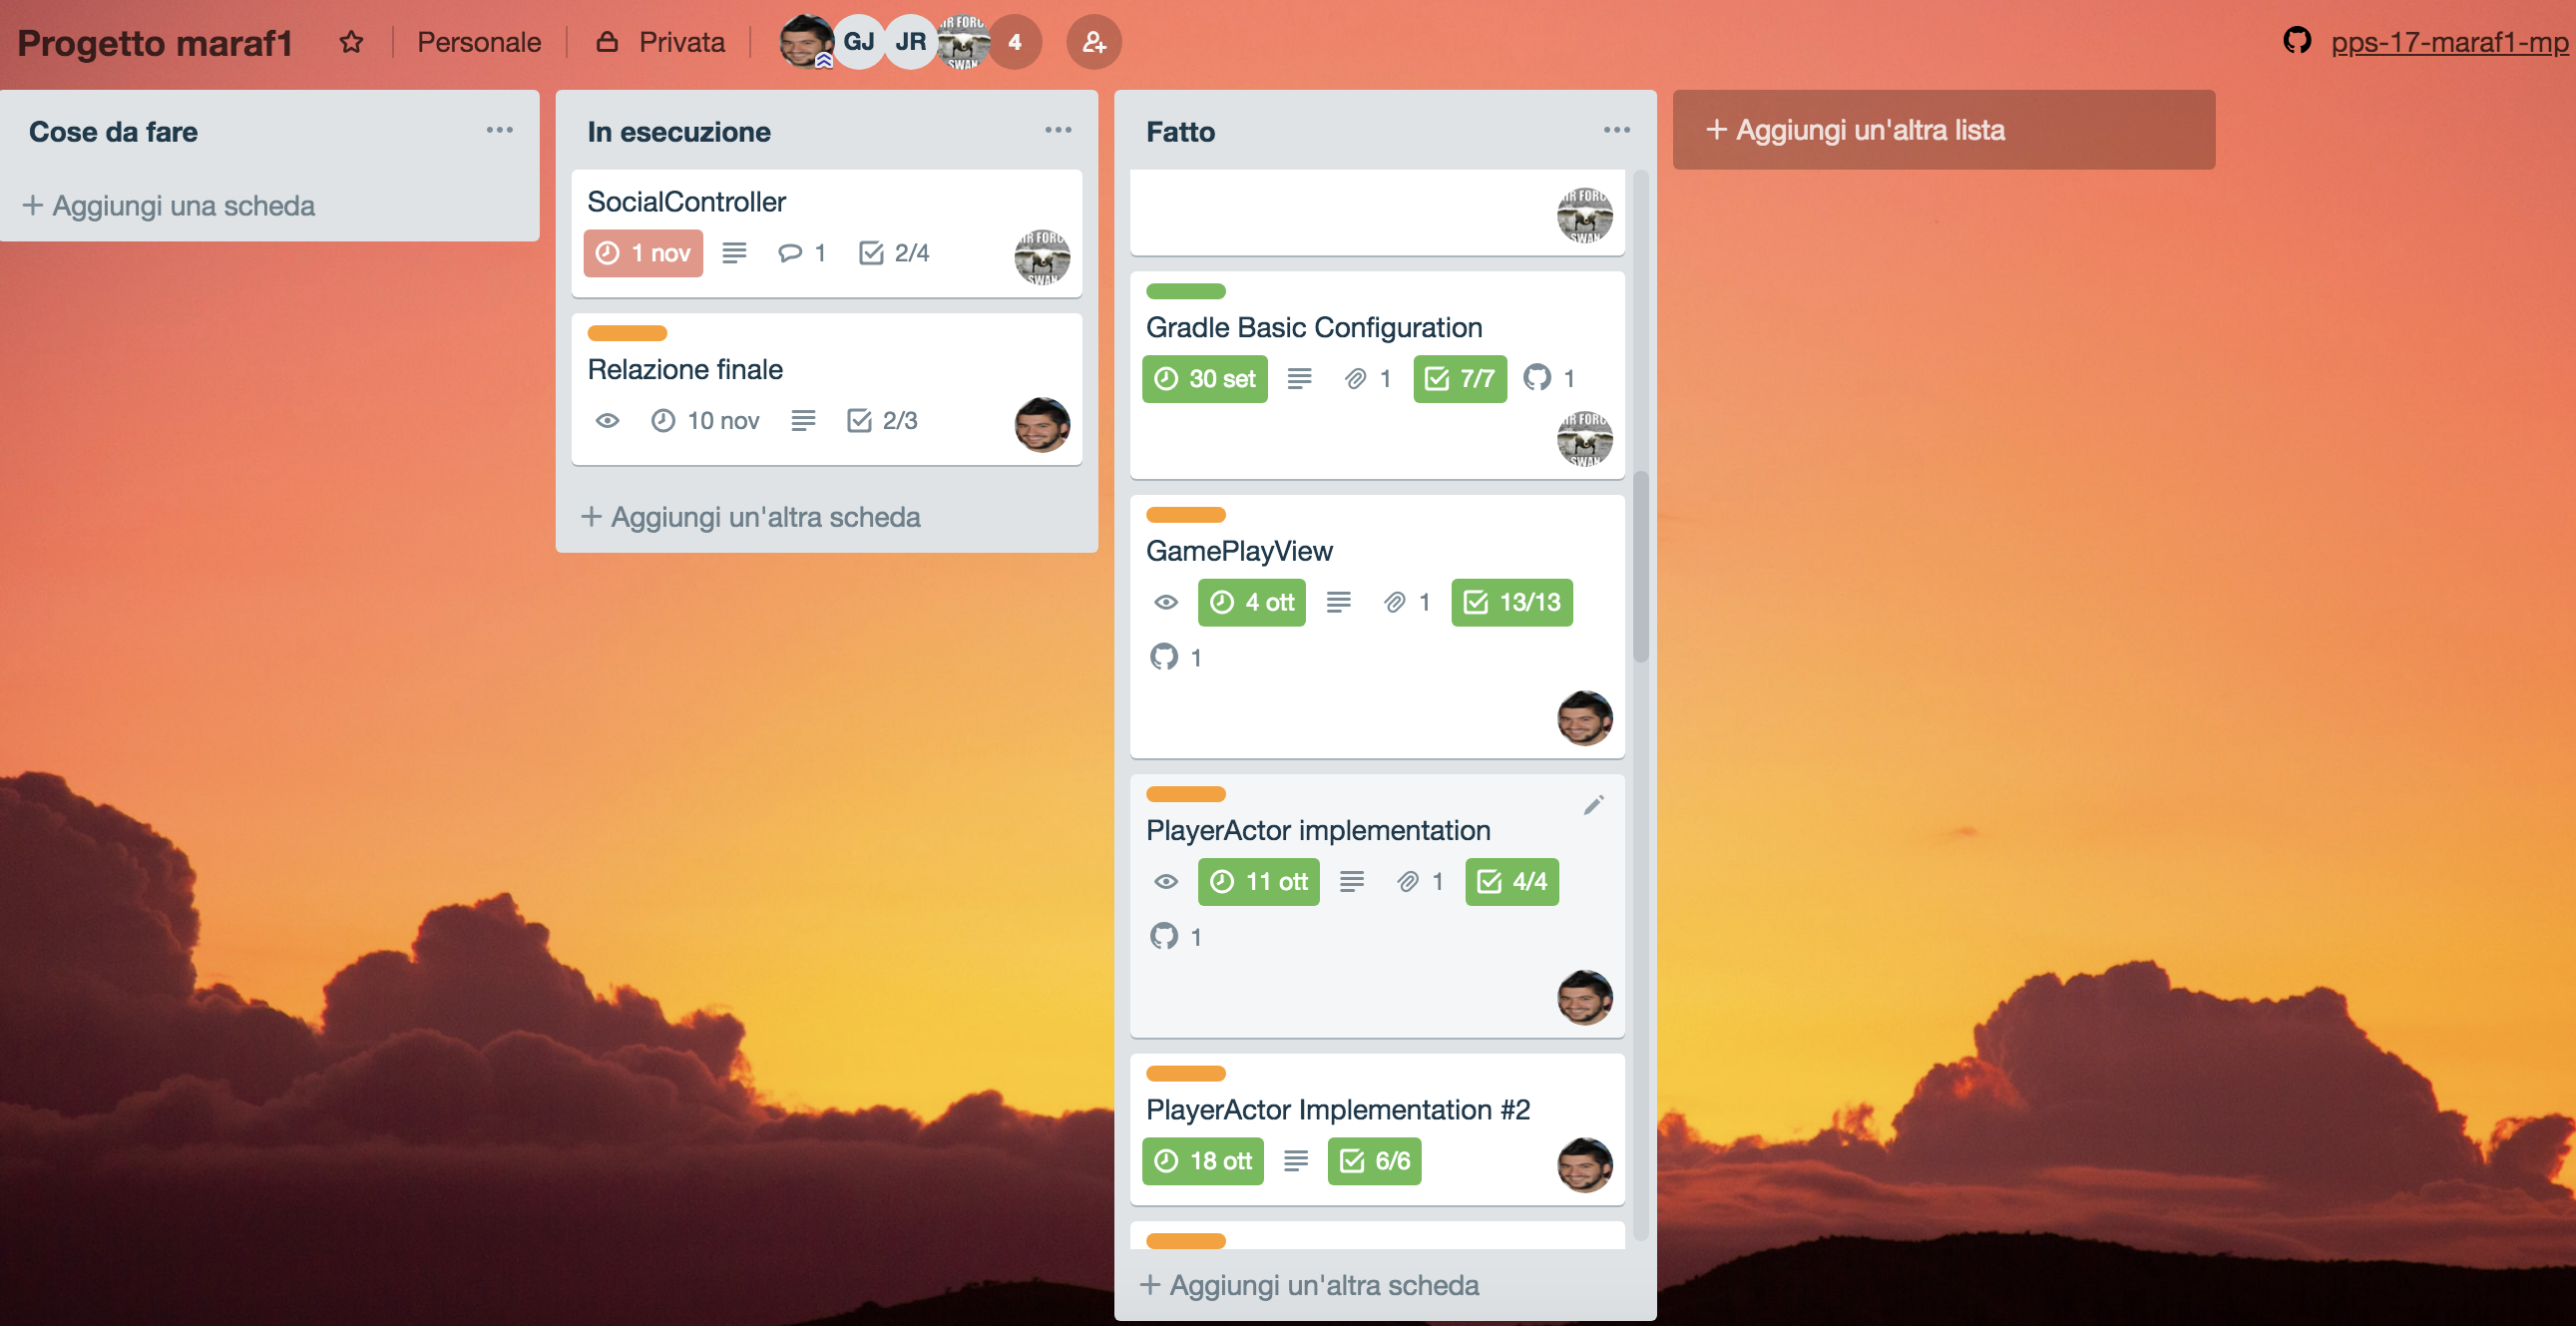
\includegraphics[width=\linewidth]{trello_dashboard.png}
 	 \caption{Dashboard di Trello.}
  	\label{fig:trello_dashboard}
	\end{figure}
  
     \clearpage
     
     \subsubsection{View}\label{subsub:brasini:view}
     Per quanto riguarda la gestione della \textbf{View}, lo studente Brasini si è occupato, nel corso delle prime due settimane di lavoro, della realizzazione dell'interfaccia grafica del gioco mediante l'utilizzo di \textbf{JavaFX}. Prima di progettare i singoli componenti all'interno della schermata però, è stata realizzata l'interfaccia \texttt{PlayGame}, implementata successivamente dal controller \texttt{PlayGameController}, che si è rivelata molto utile per poter aiutare lo studente Jakova nelle sue mansioni da Controller all'interno della suddivisione MVC. Una volta fatto ciò, lo studente ha preso familiarità con lo strumento \textit{SceneBuilder}, attraverso il quale ha realizzato l'effettiva schermata di gioco che verrà poi riutilizzata anche per le modalità di \textbf{Spettatore} e di \textbf{Replay}. Per poter visualizzare correttamente tutte le immagini della schermata, caricata da risorse esterne allo strumento utilizzato, lo studente ha dovuto studiare una modalità di caricamento che permettesse all'applicazione di poter visualizzare correttamente le immagini anche all'interno del file \texttt{.jar}. Al termine della realizzazione dell'interfaccia, lo studente si è servito dell'aiuto del plugin \textit{CheckStyle} per rimuovere tutti i \textit{warning} segnalati all'interno del codice.

	\begin{itemize}
	\item \texttt{PlayGame}.
	L'interfaccia è stata definita per poter essere implementata dal \\ \texttt{PlayGameController}. All'interno di questa interfaccia sono stati dichiarati i principali metodi come ad esempio \texttt{getCardsFirstPlayer} e \texttt{showPlayersPlayedCard} e relativa documentazione \textit{Javadoc}. In questo modo si è cercato di mantenere un certo ordine all'interno della classe \texttt{PlayGameController}, che ha implementato tutti i metodi dell'interfaccia.
	
	\item \texttt{PlayGameViewUtils}.
	All'interno di questa classe sono state inserite, sotto forma di costanti, tutte quelle variabili come ad esempio stringhe ed interi utilizzate all'interno della classe \texttt{PlayGameController} e relativi getter statici. In questo modo è stato possibile utilizzare queste variabili (che in un futuro potrebbero anche essere utilizzate da altre classi) all'interno del controller della schermata senza \textit{sporcare} il codice del controller. E' stata mostrata particolare attenzione nei confronti della pulizia del codice, considerando soprattutto l'utilizzo dei \textit{magic number}.
	
	\item \texttt{PlayGameController}.
	 Questa classe è stata, in assoluto, quella che ha richiesto maggior sforzo: da un lato è stato complicato riuscire a progettare una schermata per un'applicazione così dinamica, al cui interno  diversi componenti andavano modificati nel corso di tutta la partita, dall'altro è stato impegnativo riuscire a mantenere il codice pulito per quanto un controller di una \textit{GUI} non possa essere eccessivamente ingegnerizzato. In prima battuta, quello che è stato fatto, è stato implementare l'interfaccia \texttt{PlayGame} e i relativi metodi. A quel punto lo studente ha iniziato a lavorare attraverso lo strumento \textit{SceneBuilder} integrato all'interno dell'IDE \textit{IntelliJ}. In linea di principio, quello che è stato fatto è stato cercare da subito la possibilità di avere una schermata \textit{responsive} e che si potesse adattare alle dimensioni di qualunque schermo. Per poter ottenere questo risultato, si è scelto di avere come base un \texttt{AnchorPane} che, grazie alla sua proprietà che permette di impostare i \textit{constraint} della schermata, consentisse all'utente di poter ridimensionare la finestra a suo piacimento con il riposizionamento di tutti i componenti. Fatto ciò, lo studente ha iniziato ad implementare i componenti per la gestione delle carte: dovendo visualizzare come scoperte solamente le carte del player, si è scelto di ridurre la dimensione di quelle degli avversari e del compagno e di dare maggior risalto alle proprie. Ad ogni carta corrisponde un'\texttt{ImageView} che, se cliccata, scatena l'handler \texttt{clickedCard} che permette di comunicare l'indice della carta cliccata al controller (questi dettagli verranno trattati più approfonditamente in seguito). Ogni giocatore manterrà una lista per tutti i giocatori contenente i riferimenti alle \texttt{ImageView}. Nel momento in cui una carta viene cliccata, essa viene eliminata dalla mano dell'utente che l'ha giocata (e dunque anche dalla relativa lista) e viene posizionata in mezzo al campo, che conterrà dunque quattro ulteriori \texttt{ImageView}, una per ogni giocatore (vedi Figura 3). Inizialmente queste quattro \texttt{ImageView} saranno popolate da \textit{placeholder} che contornano la zona di nero, mentre successivamente a turno diverrà dorato nel momento in cui il relativo giocatore dovrà giocare una carta salvo poi essere rimpiazzato dalla stessa carta giocata. Dopo aver gestito e implementato la visualizzazione e gli eventi collegati alle carte, si è deciso di iniziare a lavorare sulla scelta della briscola e sulla possibilità di visualizzare, di turno in turno, la briscola corrente. Per la scelta della briscola sono stati inseriti quattro \texttt{Button} sopra alle carte del player: il click di uno dei bottoni permette la comunicazione della scelta al controller e l'immediata scomparsa dei quattro bottoni (vedi Figura 2). Dopo che la briscola è stata selezionata, verrà visualizzato un \texttt{Text} che conterrà la briscola corrente. Fatto ciò, lo studente è passato allo studio di come poter mostrare i diversi comandi all'interno della schermata. Prima di tutto sono stati aggiunti ulteriori tre \texttt{Button} che permettessero di poter selezionare il comando desiderato; successivamente sono state inserite quattro \texttt{ImageView}, una per ogni giocatore, dove verranno mostrate le immagini relative al comando selezionato (ad esempio se il player 1 cliccasse il bottone \textit{Busso}, all'interno della sua schermata verrebbe visualizzata l'immagine di una nuvoletta con all'interno il comando selezionato, mentre nelle schermate degli altri player verrebbe visualizzata la stessa immagine però in corrispondenza del giocatore che ha selezionato il comando). Fatto ciò, lo studente ha inserito delle animazioni per poter visualizzare il punteggio alla fine di ogni turno e due \texttt{Text} nella parte alta della schermata per poter visualizzare il punteggio corrente nel corso della partita, oltre ad una \texttt{ImageView} che visualizzasse, sotto forma di animazione, l'immagine di vittoria/sconfitta alla fine della partita. Infine sono stati aggiunti quattro \texttt{Text} per indicare gli username dei quattro player in partita, ed un \texttt{Text} iniziale che comunichi all'utente che si stanno ancora attendendo giocatori per poter iniziare la partita.
	
	\clearpage
	
	\begin{figure}[h!]
  	\centering
   	 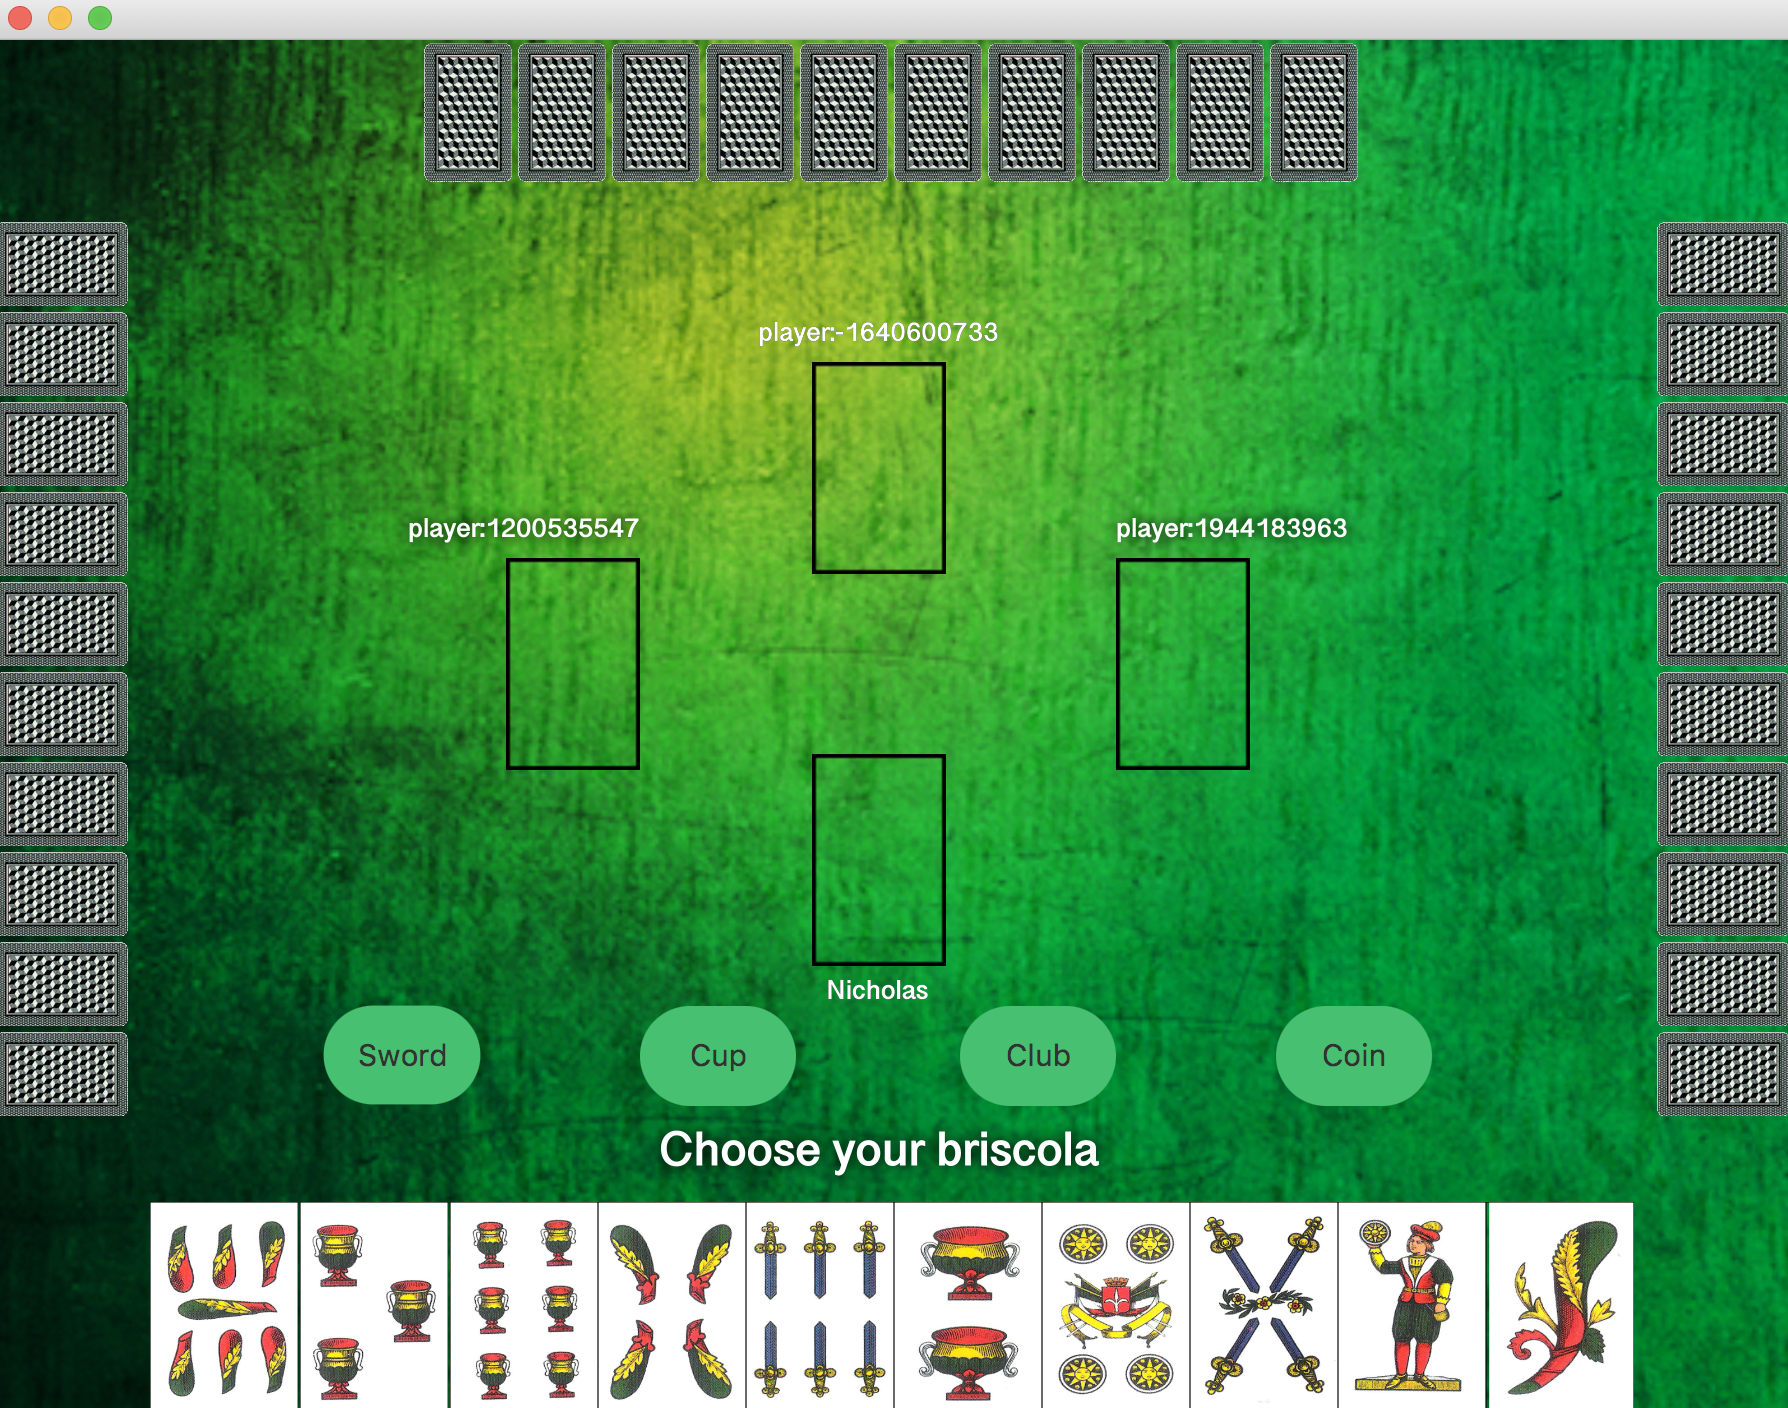
\includegraphics[width=0.8\textwidth]{playGameView1.png}
    	\caption{Scelta della briscola}
   	 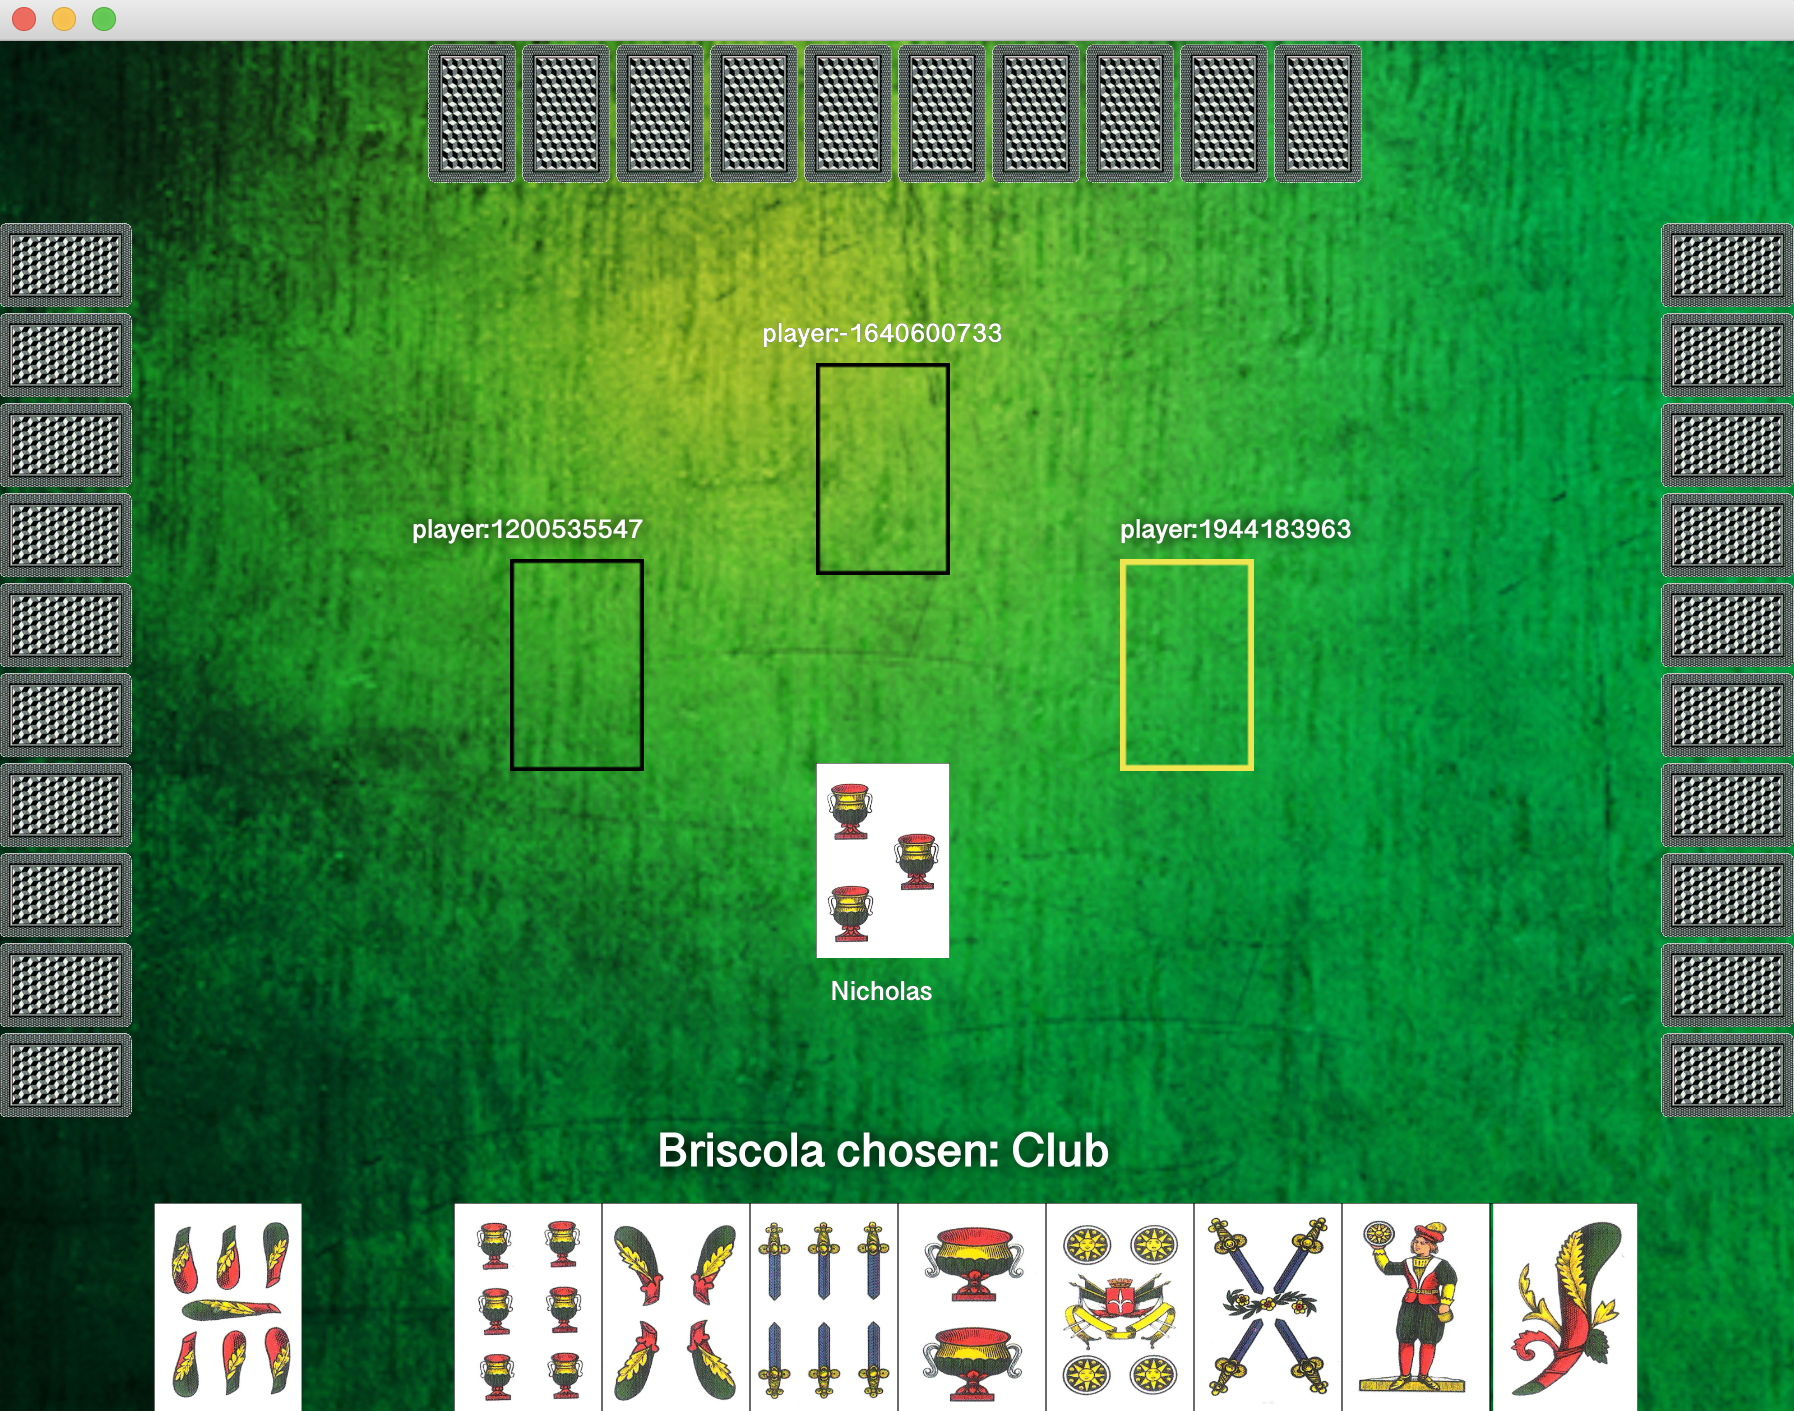
\includegraphics[width=0.8\textwidth]{playGameView2.png}
 	 \caption{Partita iniziata}
	\end{figure}
	
	\end{itemize}
     
     \clearpage
     
     
      \subsubsection{Attori}\label{subsub:brasini:actors}
     Dopo aver terminato la parte relativa alla View, lo studente Brasini, assieme al collega Jakova, si è occupato dell'integrazione totale della versione \textit{core} del gioco (di questo se ne discuterà nei paragrafi successivi relativi al lavoro svolto in cooperazione). A questo punto il team ha iniziato a lavorare alla seconda macro-fase del progetto: dopo la versione \textit{core}, il team ha iniziato ad affrontare il problema della distribuzione. Nella fattispecie, l'incarico principale assegnato a Brasini è stato quello di dover realizzare il \texttt{PlayerActorClient}, ovvero l'attore che avrebbe dovuto gestire la comunicazione con la schermata di gioco e il \texttt{GameActor}, attore realizzato dal collega Jakova che aveva come compito quello di comunicare ai quattro \texttt{PlayerActorClient} in gioco la distribuzione delle carte, il turno e tutte le altre informazioni relative alla partita. Per poter creare quest'attore, Brasini si è consultato con Jakova per un \textit{planning} piuttosto impegnativo, all'interno del quale hanno stabilito tutti i messaggi che sarebbero stati scambiati tra \texttt{PlayerActorClient} e \texttt{GameActor}. Il risultato di questa discussione ha dato vita all'oggetto \texttt{ClientMessages}. Oltre a questo, i due membri del team hanno stabilito anche di fare un uso intensivo del pattern \texttt{Publish-Subscribe} per la comunicazione tra gli attori, ma anche questa tematica sarà rinviata alla sezione in cui si discuteranno le parti sviluppate in comune. Dopo un'iniziale fase di studio, lo studente Brasini ha deciso di voler sfruttare una variante del pattern \texttt{Mediator} per poter mettere in comunicazione la GUI e l'attore: a tal proposito è stata realizzata la classe \texttt{GameController} con l'obiettivo di rendere più trasparente e pulita la comunicazione tra queste due entità. Una volta terminato il \texttt{PlayerActorClient}, lo studente Brasini ha iniziato a lavorare ad altri due attori fondamentali all'interno dell'economia del gioco. Si tratta del \texttt{ViewerActor} e del \texttt{ReplayActor}, gli ultimi due compiti che hanno impegnato lo studente prima della revisione finale delle proprie implementazioni. Come si evince dal codice, quello che è stato fatto è stato applicare il principio \textit{DRY} e il \textit{KISS}: lo studente è riuscito a riutilizzare lo stesso \texttt{GameController} sviluppato per il \texttt{PlayerActorClient} anche per gli altri due attori, a fronte di qualche piccola revisione che però non ha decisamente avuto alcun impatto pesante sulla prosecuzione del lavoro.
     
     \begin{itemize}
     \item \texttt{ClientMessages}.
     Quest'oggetto è il risultato della totalità di messaggi che vengono utilizzati dal \texttt{GameActor}, dal \texttt{PlayerActorClient}, dal \texttt{ViewerActor} e dal \texttt{ReplayActor}. Inizialmente lo studente aveva inserito all'interno del \textit{Companion Object} tutte le possibili \textit{case class} di messaggi, dal momento in cui risulta essere una \textit{best practice} nell'ambito dell'utilizzo del framework Akka. Successivamente però, essendosi reso conto che questi messaggi sarebbero dovuti essere condivisi tra più attori, si è scelto di inserirli all'interno dell'oggetto \texttt{ClientMessages}. Ogni messaggio è stato pensato per una funzionalità ben precisa e concetti che potenzialmente sarebbero potuti essere inseriti all'interno dello stesso messaggio sono comunque stati suddivisi in più messaggi per poter mantenere il codice quanto più chiaro possibile. Ogni messaggio è rappresentato all'interno di una \textit{case class} ed estende il più generico \texttt{ActorMessage}. 
     
     \item \texttt{PlayerActorClient}.
     Dopo la complessità affrontata per realizzare la GUI, è questo l'attore che ha probabilmente richiesto il maggior numero di ore prima di poter essere completato. Esso rappresenta il giocatore stesso che decide di affrontare una partita. Nel momento in cui il player decide di giocare ed apre dunque la schermata relativa ad un incontro, verrà creato di conseguenza il relativo \texttt{PlayerActorClient}, che prenderà in ingresso due parametri: il primo è l'oggetto \texttt{GameController} che servirà per comunicare i messaggi alla GUI, mentre il secondo rappresenta l'username scelto dal player. Il \texttt{PlayerActorClient} estende il \textit{trait} \texttt{ClientGameActor} e implementa la funzionalità \texttt{Stash}. Se il giocatore non si è registrato, verrà creato di default un numero random che verrà utilizzato come username del giocatore stesso. All'esterno del \texttt{PlayerActorClient} è stato realizzato un \textit{Companion Object} che contiene tre variabili intere che vengono utilizzate come costanti. Per poter ingegnerizzare al meglio questo attore, lo studente Brasini all'interno del metodo \texttt{receive}, tipico di tutti gli attori, ha inserito tutti i possibili \texttt{case} relativi ai messaggi che sarebbero potuti giungere all'attore. A questo proposito ha preferito creare dei piccoli metodi privati \textit{ad hoc} richiamati all'interno dello specifico \texttt{case} che svolgessero la reale computazione per non appesantire troppo il metodo \texttt{receive} e per mantenere più ordinato e comprensibile il codice. Come constatato in apertura del paragrafo relativo agli attori, Brasini ha fatto un uso intensivo del pattern \texttt{Publish-Subscribe} per poter dialogare in maniera nettamente più efficiente con il \texttt{GameActor}. Nel momento in cui viene istanziata la lobby infatti, l'attore riceverà un messaggio di tipo \texttt{IdChannelPublishSubscribe} che avrà come parametro l'ID della partita, che automaticamente diventerà anche l'ID del topic al quale iscriversi per poter ricevere tutte le comunicazioni dal \texttt{GameActor}. In questo modo Jakova e Brasini hanno notevolmente ridotto la complessità relativa all'invio del messaggio da parte del \texttt{GameActor} e lasciato il controllo di quali messaggi prendere in considerazione ai diversi \texttt{PlayerActorClient} sulla base del destinatario del messaggio. Una delle feature del \texttt{PlayerActorClient} era quella di, una volta ricevuto il messaggio di tipo \texttt{PlayersRef} all'interno del quale era contenuta la lista dei quattro giocatori della partita, riuscire a riordinare la lista inserendo se stesso come primo elemento e successivamente gli altri tre giocatori senza però perdere il riferimento all'ordine con il quale la lista era stata ricevuta, altrimenti sarebbero stati sbagliati gli assegnamenti del compagno e degli avversari all'interno della schermata di gioco. Per fare ciò Brasini si è avvalso dell'utilizzo del \textit{for comprehension}, zucchero sintattico per poter andare ad analizzare tutti gli elementi presenti all'interno della lista. Oltre a questo, lo studente ha fatto uso intensivo della \textit{postfix notation} dove concesso dal checker di IntelliJ, soprattutto per quanto riguarda l'invio di messaggi e la concatenazione di liste. A questo proposito si sono utilizzati con profitto anche gli \textit{impliciti} relativi ai mittenti dei messaggi di Akka, evitando ridondanti espressioni e codice superfluo ripetuto. Nel momento in cui la partita dovesse terminare, l'attore molto semplicemente invierebbe a se stesso un \texttt{PoisonPill} che in maniera del tutto trasparente gli permetterà di potersi uccidere. Nel caso in cui un player decidesse di chiudere la schermata durante una partita o nel caso in cui dovesse saltare la connessione, il risultato sarebbe la notifica di un messaggio di tipo \texttt{notifyClosedGame} nei confronti del \texttt{GameActor} che automaticamente assegnerà la vittoria al team avversario.
     
     \item \texttt{GameController}.
    Si tratta di una classe che inizialmente non era stata prevista. Essa permette di poter far dialogare in maniera del tutto trasparente il \texttt{PlayerActorClient} (ma come vedremo in seguito anche gli altri due attori) con il \texttt{PlayGameController} che gestisce la schermata di gioco. Questa soluzione prevede dunque l'utilizzo del pattern \texttt{Mediator} in una versione rivisitata, dal momento che quella originale prevederebbe l'utilizzo di due oggetti (che rappresentano le due entità che devono comunicare) all'interno del controller ma essendo inseriti nel contesto degli attori, non si è potuto realizzare per ovvi motivi un oggetto di tipo \texttt{PlayerActorClient}. La classe \texttt{GameController} viene creata nel momento in cui il player decide di giocare una partita, prende in ingresso il riferimento al \texttt{ClientController} per poter dialogare con il \texttt{PlayerActorClient} ed estende il trait \texttt{MatchController}, che a sua volta estende il trait \texttt{ActorController} il quale fornisce i due metodi che dovranno essere implementati: \texttt{createActor} e \texttt{updateGUI}. In particolare quest'ultimo metodo si è rivelato essere fondamentale dal punto di vista dell'ingegnerizzazione della classe: tutti i messaggi ricevuti dal \texttt{PlayerActorClient} infatti verranno inseriti all'interno della chiamata a questo metodo, il quale attraverso i \texttt{case} riuscirà a smistarli all'interno dei piccoli metodi privati presenti nella classe. Questa scelta è stata operata per una duplice motivazione: in primis in questo modo il codice risulta nettamente più chiaro ed ordinato, ed in secondo luogo non sarà complicato in un ipotetico futuro andare ad inserire ulteriori messaggi in invio/ricezione e relativi metodi implementativi. In sintesi questa classe permette la comunicazione tra il \texttt{PlayerActorClient} e il \texttt{PlayGameController}, senza che questi vengano mai a contatto diretto mantenendo trasparenza all'interno della comunicazione stessa (vedi Figura 4).
    
    \begin{figure}[!tbh]
    \centering
 	 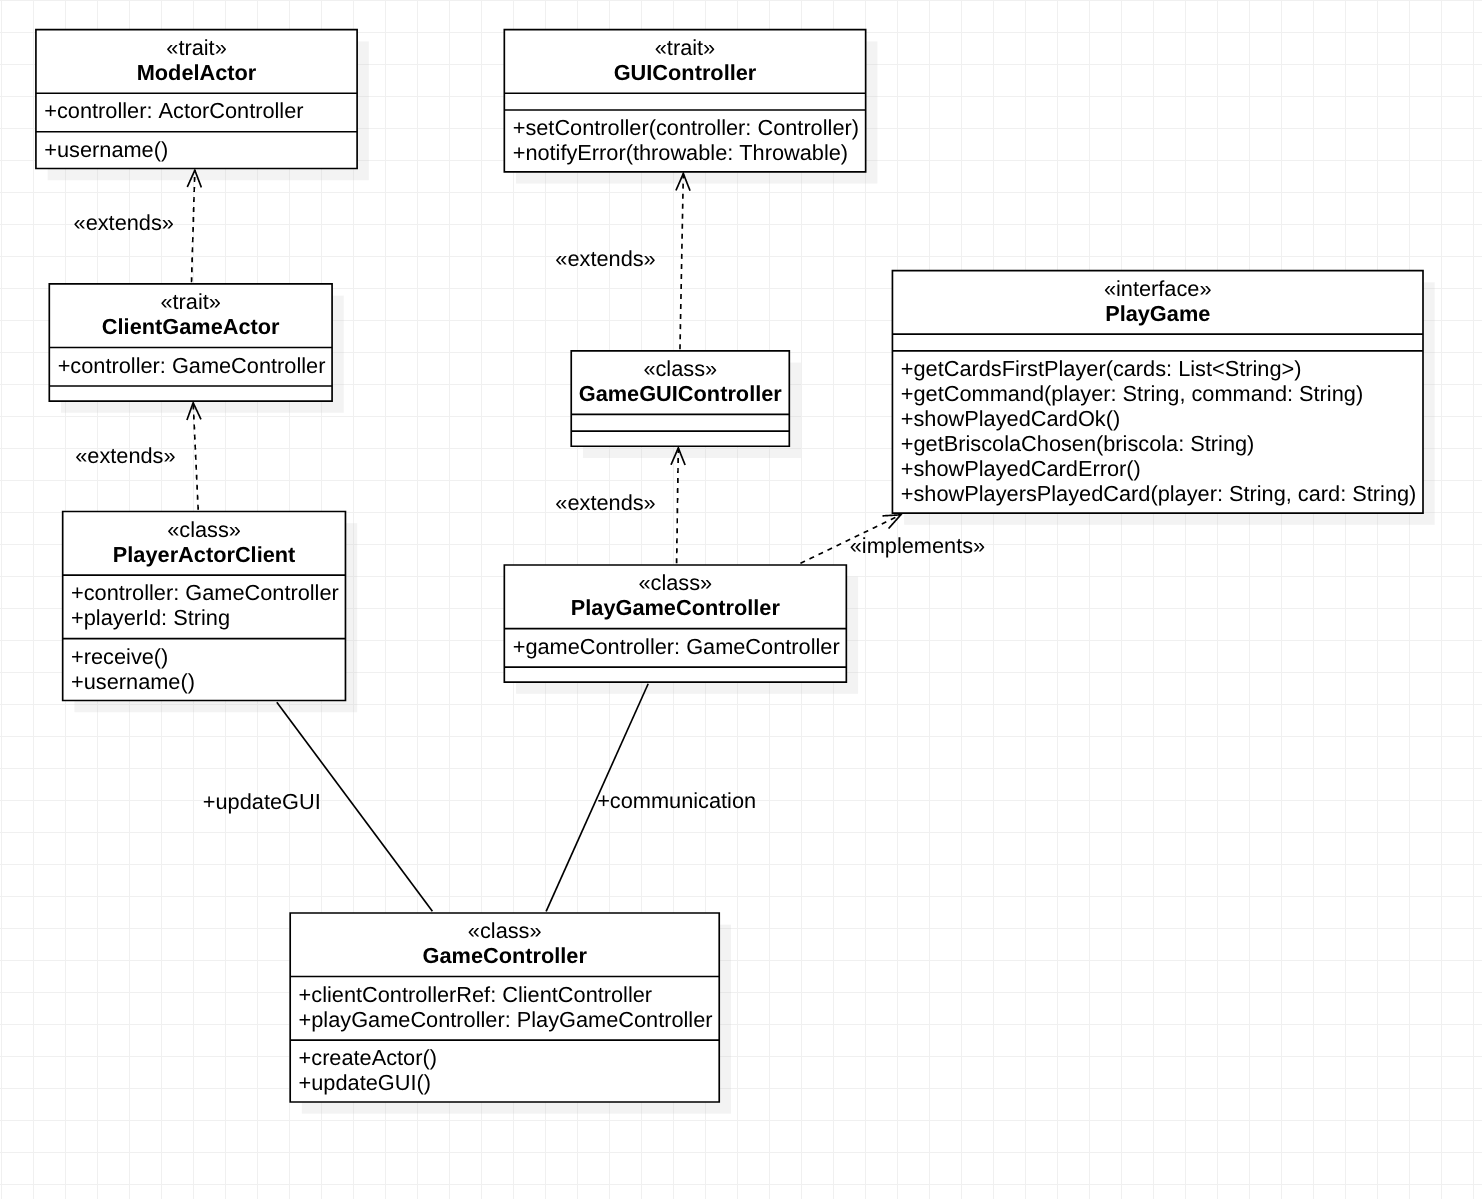
\includegraphics[width=\linewidth]{patternMediatorGameController.png}
 	 \caption{Comunicazione tra le tre entità.}
  	\label{fig:pattern_mediator}
	\end{figure}
     
     \clearpage
     
     \item \texttt{ViewerActor}.
     Giunti a questo punto, lo studente aveva già realizzato il \texttt{PlayerActorClient} e il \texttt{GameController}, senza sapere che avrebbe poi sviluppato il \texttt{ViewerActor}. Una delle sorprese più piacevoli è stata quella, dopo aver studiato per diverse ore una possibile implementazione efficiente dell'attore, di non dover creare un ulteriore \texttt{Controller} ma di poter riutilizzare il \texttt{GameController} analizzato nel paragrafo precedente. Da un lato questa soluzione si è tradotta in un minor carico di lavoro per lo studente, dall'altra ha sottolineato la bontà della costruzione del \texttt{GameController} e il suo conseguente riutilizzo. Il \texttt{ViewerActor} ha come scopo quello di gestire un player, che potrà essere loggato oppure no, che decide di prendere parte ad una partita in veste di spettatore. Verrà dunque creato nel momento in cui il player deciderà quale partita seguire (identificata da un ID) e verrà costruito passandogli un oggetto di tipo \texttt{GameController} e il suo username. Per questioni di semplicità, il giocatore non avrà la possibilità di scegliere quale player "impersonare", bensì gli verrà assegnato il primo della lista che riceverà dal \texttt{GameActor}. Esattamente come successo al \texttt{PlayerActorClient}, anche a questo attore verrà comunicato, attraverso un messaggio di tipo \texttt{IdChannelPublishSubscribe}, l'ID del canale al quale iscriversi, cosicché attraverso il pattern \texttt{Publish-Subscribe} possa seguire ogni mossa dei giocatori impegnati nella partita e notificarla al proprio \texttt{GameController}. Il vero problema di questo attore, che lo differenzia rispetto ad un player classico, è il seguente: esso può decidere di visualizzare una partita che è già cominciata, per cui al contrario dei \texttt{PlayerActorClient} dovrà poter inserirsi all'interno della stessa partita ricevendo un messaggio che vada ad effettuare un \textit{recap} della situazione attuale, come ad esempio le carte rimaste in mano ai giocatori, il punteggio e la briscola corrente. Per risolvere questo problema, lo studente ha deciso di costruire un nuovo tipo di messaggio, il \texttt{RecapActualSituation}, che comunicasse all'attore la situazione della partita. Fino a quando l'attore non avesse ricevuto quel tipo di messaggio, non avrebbe potuto comunicare alcuna informazione al proprio \texttt{GameController} sebbene fosse in ascolto sul canale della gara. Per poter risolvere questa situazione con una soluzione brillante, Brasini ha deciso di servirsi del costrutto \texttt{become}, che permette all'attore di rimanere in attesa di uno specifico messaggio e, solamente una volta ricevuto, poter procedere e prendere in considerazione anche altre tipologie di messaggi (vedi Figura 5). Così come successo con il \texttt{PlayerActorClient}, anche in questo caso lo studente ha preferito separare l'implementazione (inserita all'interno di specifici micro-metodi) dalla ricezione dei messaggi all'interno della \texttt{receive} dell'attore per mantenere più ordinato, pulito e comprensibile il codice. 
     
     
         \begin{figure}[!tbh]
    \centering
 	 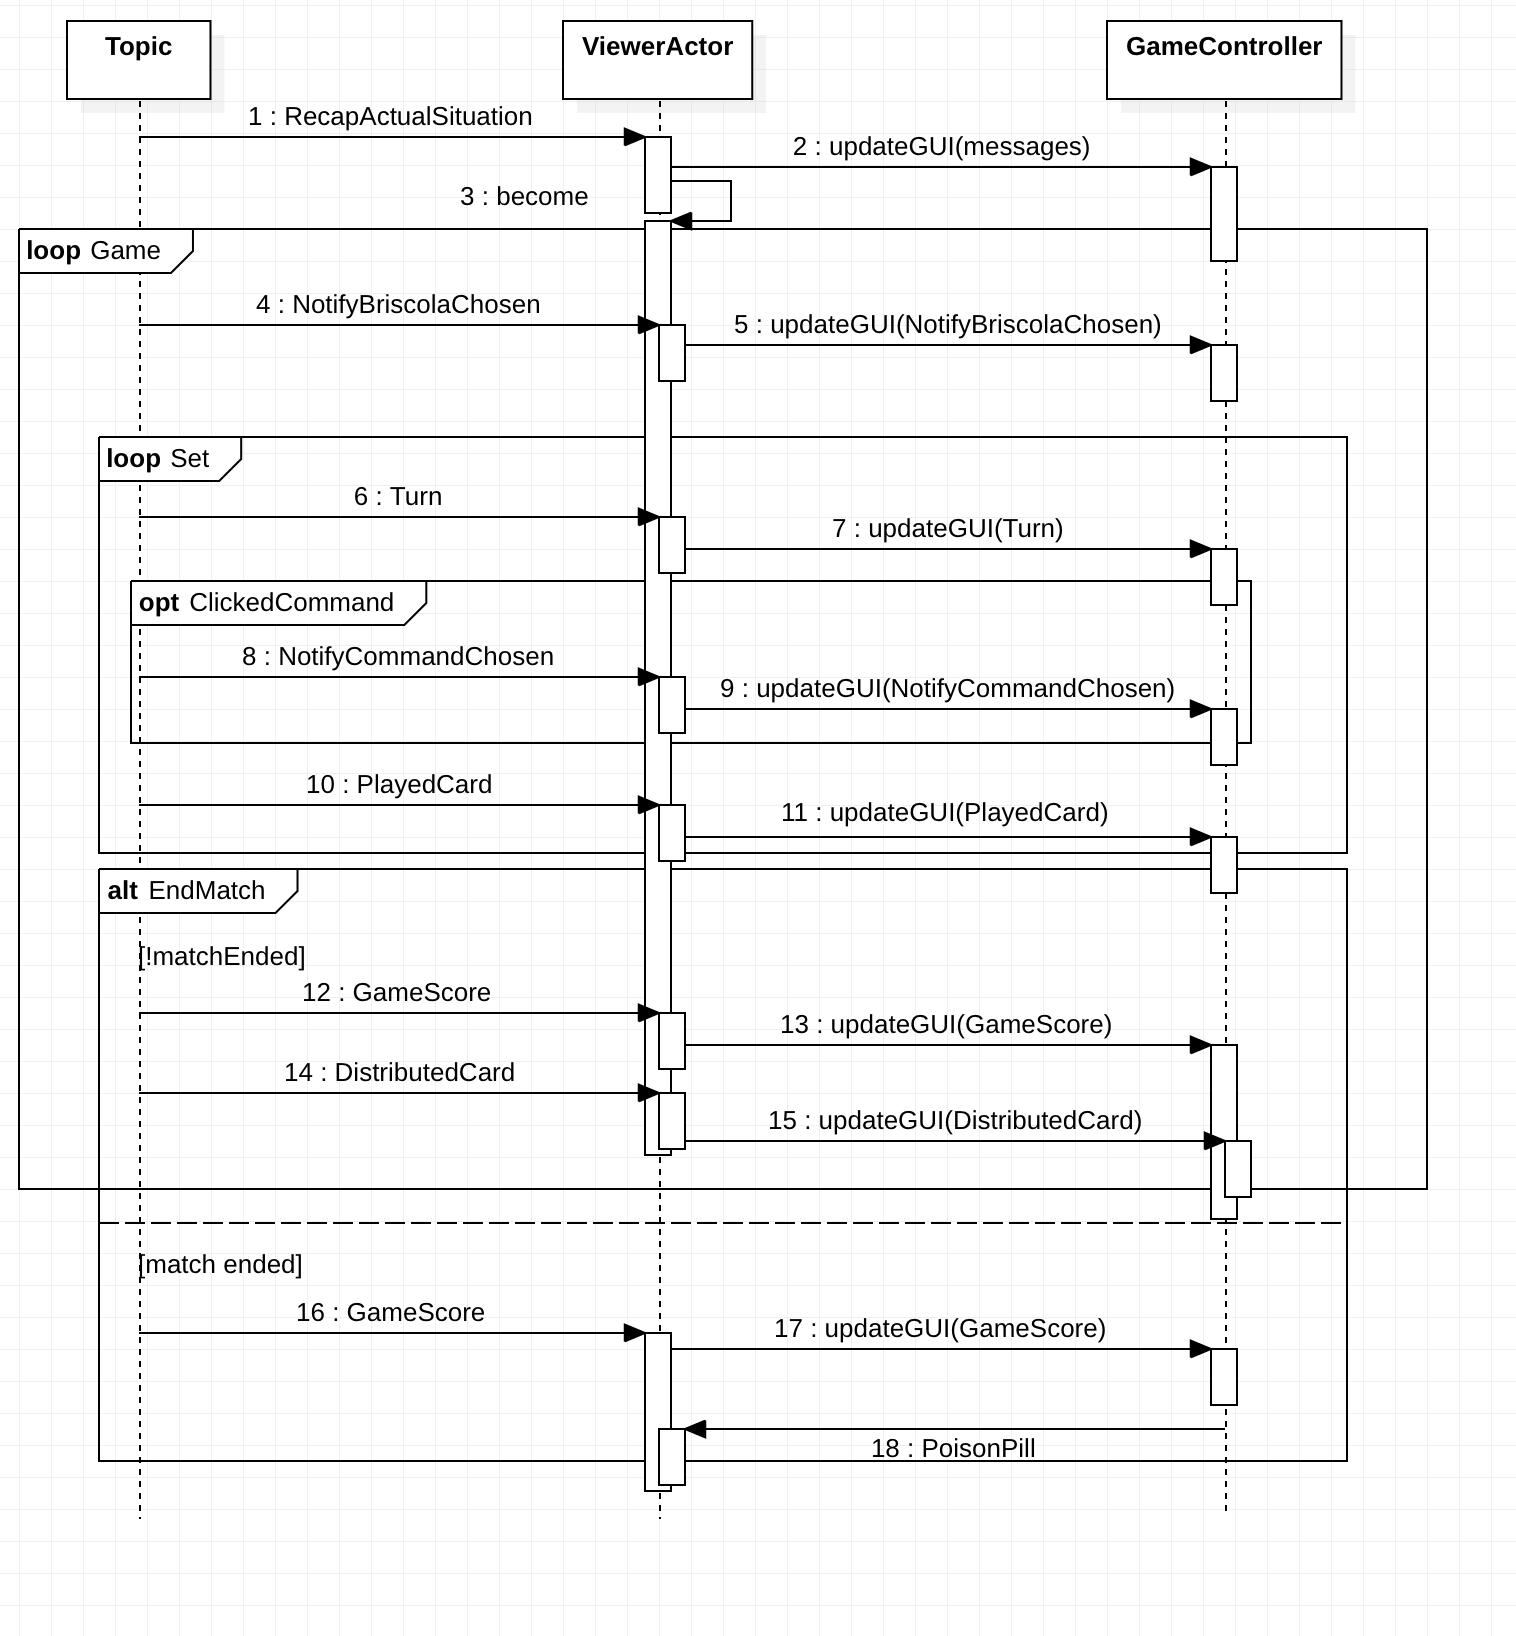
\includegraphics[width=\linewidth]{sequenceDiagramViewerActor.png}
 	 \caption{Sequence diagram del ViewerActor}
  	\label{fig:viewer_actor}
	\end{figure}
	
	
	\clearpage
	
	     
     \item \texttt{ReplayActor}.
     L'ultimo impegno implementativo per lo studente è stato quello del \\ \texttt{ReplayActor}. La costruzione dell'attore è stata abbastanza simile a quella dei due precedenti attori, ma in questo caso si è dovuto risolvere il problema di come visualizzare il replay. Le possibilità ipotizzate erano due: o inserire all'interno della schermata un bottone che, ogni volta premuto, avrebbe mandato avanti il gioco di una mossa, oppure utilizzare uno \textit{scheduler} interno predefinito che esortasse l'attore a inviare, ogni tot millisecondi, il messaggio relativo alla mossa eseguita al \texttt{GameController} che l'avrebbe poi notificata al \texttt{PlayGameController}. Alla fine lo studente ha optato per la seconda possibilità dopo aver studiato e imparato ad implementare lo scheduler interno di \textbf{Akka}: esso richiede di impostare il momento in cui partire, il messaggio da inviare all'attore e l'intervallo di tempo ogni cui questo messaggio deve essere inviato. In fase di costruzione l'attore prendeva in ingresso l'oggetto \texttt{GameController}, il proprio username e l'oggetto di tipo \texttt{Game}, il vero contenitore di tutte le mosse della partita salvata su database. L'unico messaggio che l'attore era predisposto a ricevere era un messaggio di tipo \texttt{SendHeartbeat}, inserito come case class all'interno del \textit{Companion Object} dell'attore insieme ad altre costanti utilizzate in seguito. Questo tipo di messaggio, abbinato ad un \textit{pattern matching} su una variabile di tipo \texttt{ReplayActorStatus} inizializzata a \texttt{PRE\_SET}, permetteva di capire quale dei metodi dell'attore andare a richiamare. Ancora una volta, per avere una maggior chiarezza e un codice più pulito possibile, si è scelto di realizzare un oggetto \texttt{ReplayActorStatus} al cui interno sono stati definiti dei \textit{case object} che rappresentassero lo stato del contatore. I possibili stati erano:
     
     \begin {itemize}
   
     \item \texttt{PRE\_SET}. Questo stato rappresentava lo stato iniziale in cui l'attore doveva ricadere per poter iniziare il replay della partita. All'interno della \texttt{receive}, se il \texttt{gameCounter} fosse risultato essere uguale a questo stato, sarebbe stato chiamato il metodo \texttt{computePreSet} (e così anche per gli stati successivi che richiameranno i relativi metodi). All'interno di questo metodo si sarebbe andato ad analizzare l'oggetto di tipo \texttt{Game} passato come parametro all'attore e si sarebbe ricavata la lista dei quattro giocatori della partita, inviata poi al \texttt{GameController} secondo le modalità analizzate in precedenza. Fatto ciò, si sarebbe impostato il contatore allo stato successivo.
   
     \item \texttt{START\_SET}. Questo stato è quello che rappresenta la fase successiva dello stato \texttt{PRE\_SET}. In virtù di questo stato verranno recuperati i punteggi del turno di entrambi i team, la briscola corrente e tutte le carte in mano al player che questo attore impersona. In quest'ultimo passaggio si è resa necessaria la creazione del path della carta per poter inviare al \texttt{GameController} una lista dei path delle carte in mano al primo player, così da essere pronte per essere caricate all'interno della schermata di gioco. Nel metodo relativo a questo messaggio, il \texttt{computeStartSet}, verranno dunque inviati al \texttt{GameController} la briscola, le carte del primo giocatore e i due punteggi del turno. Fatto ciò, verrà incrementato il contatore che passerà allo stato successivo e infine verranno incrementate anche le variabili relative alle mani e ai turni, cosicché al turno successivo si potrà procedere con l'acquisizione delle nuove giocate.
     
   \item \texttt{TURN\_SET}. Questo stato rappresenta la fase successiva dello stato precedente. In questo caso verrà invocato il metodo \texttt{computeTurnSet} al cui interno verrà inviato al \texttt{GameController} il messaggio relativo a quale giocatore dovrà giocare la prossima carta. Fatto questo, si imposterà lo stato a quello successivo.
     
     \item \texttt{MIDDLE\_SET}. In virtù di questo stato verrà invocato il metodo \texttt{computeMiddleSet}, che avrà come compito quello di recuperare la carta giocata da un giocatore, convertirla in path ed inviarla al \texttt{GameController}. Fatto ciò, si cercherà di incrementare la mossa successiva: se questa risultasse essere vuota, allora si imposterà il contatore allo stato \texttt{TURN\_SET} per poter procedere con il nuovo set; se anche questa operazione non fosse portata a termine, significherebbe che sono già state giocate le quaranta carte di quel turno e allora si imposterebbe il contatore allo stato \texttt{END\_SET}.
     
     \item \texttt{END\_SET}. Si verrà a contatto con questo stato ogni qualvolta verranno giocate quarantra carte. Verrà chiamato il metodo \texttt{computeEndSet} che tenterà di incrementare la variabile relativa al turno per passare al successivo. Se questa operazione verrà portata a termine, allora significa che la partita non è ancora finita, si invierà un messaggio con i due punteggi al \texttt{GameController} e si imposterà il contatore a \texttt{START\_SET} per cominciare il nuovo turno. In caso contrario, significa che la partita è terminata, per cui si invierà un messaggio al \texttt{GameController} segnalando il team vincitore della partita. In questo caso verrà impostato il contatore a \texttt{END\_GAME}.
     
     \item \texttt{END\_GAME}. Si tratta dell'ultimo stato disponibile, che rappresenta la fine della partita. Nel momento in cui verrà invocato il relativo metodo \texttt{computeEndGame}, quello che farà l'attore sarà semplicemente inviarsi un messaggio di tipo \texttt{PoisonPill} per uccidersi. A quel punto la schermata del Replay verrà chiusa e si tornerà alla precedente.
     
     
          \end{itemize}
     
    
     \end{itemize}
     
     
     
     
     \clearpage
        \subsection{Gjulio Jakova}\label{subsec:jakova}

 Per quanto riguarda il progetto \textbf{Maraph-1}, lo studente \textbf{Gjulio Jakova} ha sviluppato le seguenti parti in maniera autonoma:
        
        \begin{itemize}
        \item \textbf{Core}
        		\begin {itemize} 
		\item 	Controller e implementazione di \texttt{Player}(Model) in una prima versione non-distribuita del gioco.
     	\end {itemize}
     
     	\item \textbf{Server}
		\begin {itemize}
		\item Creazione attore \texttt{GameActor} per la gestione di tutte le partite.
		\item Adattamento del pattern \texttt{Distributed Publish-Subscribe} nel Cluster e gestione dello stashing dei messaggi nel \texttt{GameActor} e \texttt{PlayerClientActor}.
	\end {itemize}
	
	\item \textbf{View}
		\begin {itemize}
		\item Implementazione della schermata iniziale di autenticazione (login e registrazione).
		\item Implementazione della schermata dell’utente loggato.
		\item Implementazione della schermata dell’utente non-loggato.
		\item Caricamento di tutte le risorse grafiche per le tre schermate precedenti.
		\item Aggiunta di stile ai componenti di ciascuna schermata.
		\end{itemize}
		
     \end {itemize}

 \subsubsection{Core}\label{subsub:jakova:core}
    Nel primo sprint dove l’obiettivo principale era la realizzazione di una prima versione non-distribuita del gioco con tutte le regole di Marafone seguendo il pattern\texttt{ MVC}, lo studente Jakova si è occupato del Controller e dell’implementazione del \texttt{Player} nel Model. Nel Controller il compito era gestire gli eventi che arrivavano dalla View come la carta scelta, la scelta della briscola, i comandi scelti dai giocatori (busso, striscio o volo) eseguendo delle operazioni che potevano interessare al Model. Lo stesso discorso anche dall’altro lato, dove il Model forniva dei dati da comunicare alla View per esempio: la distribuzione delle carte, i turni, il vincitore della mano ecc. 

 \subsubsection{Server}\label{subsub:jakova:server}
A partire dal secondo sprint, dove l’obiettivo era che il sistema avesse un’architettura distribuita, lo student si è occupato della creazione dell’attore \texttt{GameActor}. L’attore \texttt{GameActor} viene creato appena dentro la lobby ci sono i quattro giocatori, e permette di gestire più partite in contemporanea, ovvero ogni partita sarà gestita da un singolo GameActor. Valutando bene quale poteva essere la scelta giusta per la comunicazione real-time server-client (\texttt{GameActor} – \texttt{PlayerClientActor}) si è deciso di utilizzare gli strumenti che \textbf{Akka Cluster} metteva a disposizione. Questa scelta è stata fatta anche per il fatto che il toolkit \textbf{Akka} lo conoscevamo già. L’altro motivo era anche per il fatto che il clustering porta la trasparenza della posizione al livello successivo. L'attore potrebbe esistere localmente o in remoto e potrebbe risiedere ovunque nel cluster; il nostro codice non deve preoccuparsi di questo. Invece per lo scambio di messaggi tra gli attori è stato deciso di utilizzare il design pattern \textbf{Publish/Subscribe} che ci forniva un approccio di notifica/comunicazione asincrona fra i diversi attori. Il funzionamento del pattern \textbf{Publish/Subscribe} è semplice: mittenti e destinatari di messaggi dialogano attraverso un \textit{topic}(canale), al quale bisogna iscriversi per poter ricevere i messaggi. Il mittente di un messaggio (detto \textit{publisher}) non deve essere consapevole dell'identità dei destinatari (detti \textit{subscriber}); esso si limita a "pubblicare" il proprio messaggio nel topic. Nel caso di Akka quello che fa da tramite viene chiamato \textit{mediator}. Un subscriber è libero di “abbonarsi” alla ricezione di messaggi aventi certe caratteristiche. Questo schema implica che ai publisher non sia noto quanti e quali siano i subscriber e viceversa. Questo può contribuire alla scalabilità del sistema. Nel nostro caso questo pattern è stato molto utile poiché avevamo un \texttt{GameActor}(responsabile della partita) che aveva il ruolo di publisher e altri attori come \texttt{PlayerClientActor}(responsabile di un singolo giocatore), \texttt{ViewerActor}(responsabile del giocatore spettatore) che avevano il ruolo di subscriber e che si mettevano in ascolto sul canale, aspettandosi tipi di messaggi diversi, in attesa che il \texttt{GameActor} comunicasse qualcosa. Il pattern ci ha permesso che il \texttt{GameActor} non mandasse ogni volta un messaggio a ciascun giocatore, quindi in totale quattro messaggi ogni volta, ma soltanto un messaggio che tutti i giocatori che erano in ascolto sul topic lo ricevessero. Un altro problema negli attori era la sequenza precisa dei messaggi che doveva ricevere, ossia quando l'attore è in attesa di qualcosa da completare prima di elaborare il prossimo messaggio. In Akka, lo \textit{stashing} dei messaggi consente a un attore di bufferizzare temporaneamente tutti o alcuni messaggi che non possono o non devono essere gestiti utilizzando il comportamento corrente dell'attore. Nel nostro caso per fare sì che tutti i giocatori (attore e view corrispettivo) siano allo stesso passo, abbiamo introdotto un altro tipo di messaggio di conferma (\texttt{Ack}) in modo che il \texttt{GameActor} non possa andare avanti senza aver ricevuto la conferma che tutti i giocatori hanno ricevuto il messaggio e che nessun messaggio sia perso. 

\begin{figure}[h!]
 \centering
  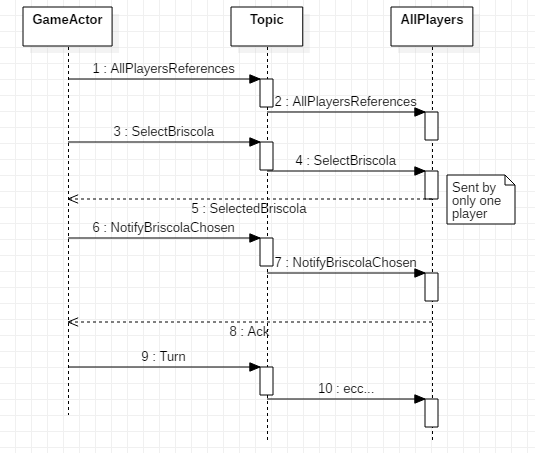
\includegraphics[width=0.7\textwidth]{actorsMsgSeq.png}
   \caption{Un esempio della sequenza di scambio dei messaggi}
\end{figure}

Sempre nel \texttt{GameActor} viene gestita la creazione un messaggio di \textit{recap}, contenente una serie di strutture dati, che servirà al \texttt{ViewerActor} per essere aggiornato con le mosse fatte prima che lui cominci a guardare la partita. Lo studente ha fatto uso del pattern \texttt{Strategy} nei metodi \textit{impliciti} (per esempio nel metodo che restituisce alla view i path di tutte le carte da poter visualizzare), di \texttt{PartialFunction} (nella receive dei messaggi). Sono state utilizzate anche funzionalità avanzate di Scala, come la \textit{for comprehension}, \textit{postfix notation}(nell'invio dei messaggi) ed il \textit{pattern matching} per rendere il codice il più semplice e leggibile possibile.

 \subsubsection{View}\label{subsub:jakova:view}
    La view è stata realizzata utilizzando la libreria grafica \textit{JavaFX}, dove le diverse schermate sono state definite attraverso l’utilizzo dei file \textbf{.fxml} (linguaggio XML-based) che fornisce la struttura per costruire un'interfaccia utente separata dalla logica dell'applicazione del nostro codice. Ho realizzato la schermata di autenticazione dove login e registrazione si trovano all’interno di un unico \textit{Scene}, che è composta da semplici componenti di input, label e bottoni. In base alle risposte restituite dalle \textit{REST API} vengono mostrate alert di informazione (in caso di successo) e alert di errore (in caso di fallimento). 

Per quanto riguarda la gestione della logica di controllo della schermata, è stata definita la classe \texttt{RegistrationLoginController} in modo che la logica di controllo sia separata dall’implementazione della view stessa. All’interno di questa classe sono stati definiti tutti i comportamenti che si devono applicare al verificarsi di determinati eventi. 

\begin{figure}[h!]
 \centering
  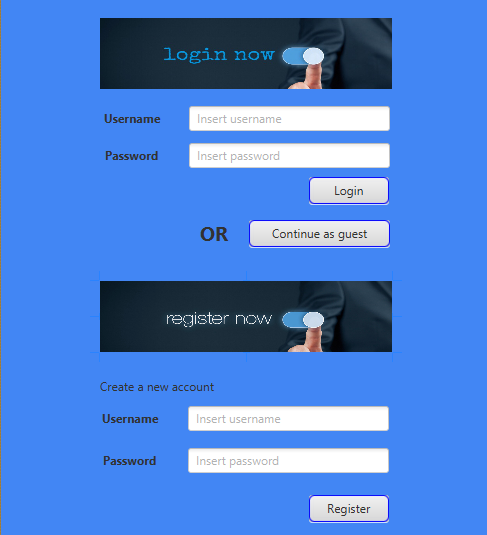
\includegraphics[width=0.65\textwidth]{login.png}
   \caption{Schermata iniziale}
\end{figure}

Poi lo studente ha realizzato anche le due schermate dell’utente loggato e non-loggato. Un utente loggato può giocare in modo \textit{competitivo} (con effetto sulla classifica) e \textit{non-competitivo} (nessun effetto sulla classifica), guardare una partita già finita (replay della partita), guardare una partita da spettatore, visualizzare la lista degli amici ed altri giocatori online, inviare una richiesta di amicizia, invitare un amico a giocare come partner o come avversario. Invece un utente non-loggato può soltanto giocare in modo non-competitivo e guardare una partita da spettatore. 

\begin{figure}[h!]
 \centering
  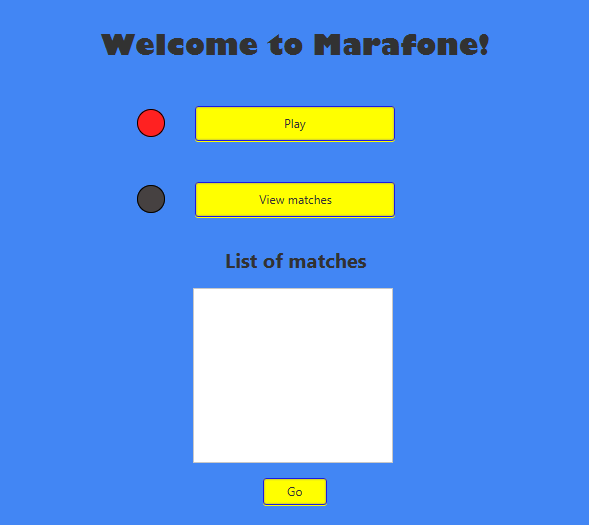
\includegraphics[width=0.8\textwidth]{generic.png}
   \caption{Schermata dell'utente non-loggato }
\end{figure}

Componenti principali della scena sono bottoni, listView e comboBox che inizialmente non sono tutti visibili. In base a determinate situazioni certi componenti si abilitano o disabilitano in modo da evitare di avere più schermate. 
L’invio dell’amicizia o dell’invito per giocare scatena nella GUI dell’utente invitato un alert di conferma. In base alla risposta l’invitante vedrà apparire nella sua GUI una label con risposta che scompare dopo 5 secondi (con una chiamata asincrona per non bloccare la GUI).

Anche qui la logica di controllo delle schermate è definita nelle classi \texttt{GenericGUIController} e \texttt{SocialGUIController} che gestiscono tutti i vari comportamenti che si devono applicare al verificarsi di determinati eventi. Entrambe le classi implementano l’interfaccia \texttt{BasicPlayerOptions} contenente le operazioni in comune che hanno i diversi tipi di utenti.

Lo studente si è occupato anche di aggiungere lo stile a tutti i componenti delle varie schermate realizzate, in modo da avere un’interfaccia grafica attraente, semplice da usare e molto intuitiva grazie anche ai colori associati ai componenti (bottone e comboBox stesso colore). Questo è stato realizzato grazie a \textit{JavaFX} che permette di aggiungere lo stile \textit{CSS} a tutti i componenti.

\begin{figure}[h!]
 \centering
  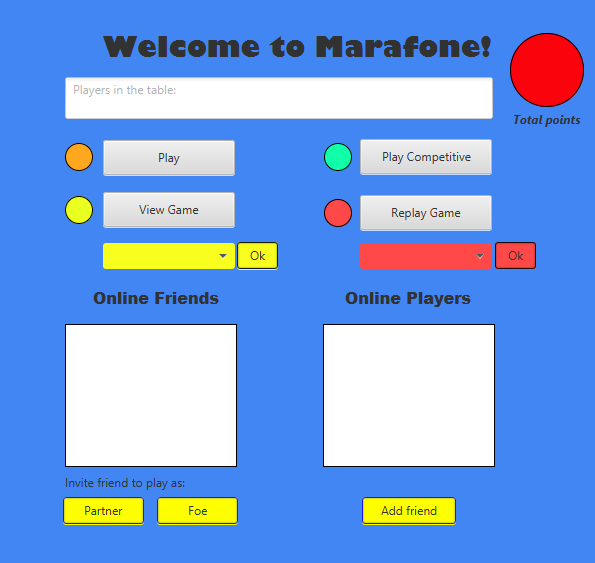
\includegraphics[width=0.8\textwidth]{social.png}
   \caption{Schermata dell'utente loggato }
\end{figure}

        \subsection{Federico Naldini}\label{subsec:naldini}
        \subsection{Jacopo Riciputi}\label{subsec:riciputi}
        
        \clearpage
        
        \subsection{Componenti creati in cooperazione}\label{subsec:cooperation}
        Nel corso dello sviluppo di questo progetto, è capitato che due membri abbiano dovuto interagire per poter integrare quanto sviluppato fino a quel momento o semplicemente per poter prendere delle decisioni che avrebbero avuto un impatto deciso sullo sviluppo futuro del proprio codice. Di seguito elenchiamo le principali attività di coordinazione tra i membri del team.
        
        
        \subsubsection{Brasini e Jakova}\label{subsub:cooperation:brasinijakova}
        Gli studenti Brasini e Jakova hanno collaborato alle seguenti parti:
        
        \begin {itemize}
        \item \textbf{Integrazione della versione core}. Gli studenti, terminati gli sprint relativi alla versione core, hanno preso in mano tutto il progetto integrando tra loro le diverse parti di codice prodotte dai quattro membri del team. Grazie al \textit{testing} effettuato hanno potuto constatare la correttezza della versione core e l'hanno pubblicata sul branch \texttt{master}.
        \item \textbf{Planning per la realizzazione dell'oggetto \texttt{ClientMessages}}. E' stata una fase piuttosto lunga, durante la quale i due studenti hanno collaborato per valutare quali fossero i messaggi più appropriati e comuni da dover inserire all'interno dell'oggetto \texttt{ClientMessages}. Si è deciso di realizzare un oggetto comune dal momento in cui sia il \texttt{GameActor}, ad opera di Jakova, che \texttt{PlayerActorClient, ViewerActor e ReplayActor} sviluppati da Brasini avevano una forte interazione e un continuo scambio di messaggi.
        \item \textbf{Realizzazione del canale di comunicazione tra attori mediante pattern \\ \texttt{Publish-Subscribe}}. Si è deciso di sfruttare questo particolare pattern che ha permesso ai due studenti di semplificare enormemente la vita dei propri attori. Grazie al canale realizzato, il \texttt{GameActor} ha avuto la libertà di comunicare i messaggi diretti a tutti i player (e ad eventuali viewer) un'unica volta. La scelta se considerare i messaggi oppure meno pertanto è stata presa dagli altri tre attori in gioco, che sulla base del player di destinazione dei diversi messaggi hanno deciso se ricevere il messaggio oppure scartarlo.
        \item \textbf{Gestione dello stash dei messaggi tra gli attori e relativi ACK di conferma}. I due studenti, in conclusione, hanno notato che, a causa di possibili ritardi della rete, bisognava poter gestire le situazioni pericolose. Il principale problema è stato arginato utilizzando messaggi ACK di conferma: ad esempio nel \texttt{PlayerActorClient} nel momento in cui viene comunicata sul canale la briscola del turno, bisognava rispondere al \texttt{GameActor} con un messaggio di tipo \texttt{BriscolaACK} per confermare l'avvenuta ricezione dello stesso messaggio. Fino a quando il \texttt{GameActor} non avesse ricevuto tutte e quattro le conferme, non sarebbe andato avanti con l'invio dei messaggi successivi. In questo modo è stato prevenuto anche il fatto che le conferme stesse potessero ritardare: in quel caso in realtà il problema non si pone, poiché fino a quando il \texttt{GameActor} non avesse ricevuto le conferme, non avrebbe fatto nulla. Oltre alle conferme è stato utilizzato anche il meccanismo dello \texttt{stash}, in particolar modo nella situazione in cui il player avesse dovuto decidere la briscola senza però aver ancora ricevuto il messaggio contenente le sue carte. Per evitare di far scegliere la briscola senza poter nemmeno osservare le proprie carte, si è deciso di \textit{stashare} il messaggio fino a quando non fosse giunto quello contenente le carte. A quel punto si sarebbe proceduto con la \texttt{unstashAll} per poter riprocessare il messaggio relativo alla scelta della briscola.
   	\end {itemize}
        
        \clearpage
        
 \section*{\Huge {\textbf Capitolo 6}\label{chapter6}}
    \section{Retrospettiva}\label{sec:retrospective}
\subsection{Andamento degli sprint}
A progetto concluso possiamo per certo dire di essere abbastanza soddisfatti con l’andamento del progetto in generale. Siamo partiti inizialmente un po’ lenti per vari motivi però questo non ci ha penalizzati per concludere con successo il tutto, anzi ci ha spinto successivamente di dare di più. 
Avendo adottato un approccio Agile simil Scrum  ci ha facilitato molto il lavoro in team, permettendoci di avere dei risultati immediati e costante miglioramento del prodotto in periodi brevi. Tale approccio permette di essere sempre in contatto diretto e immediato con tutti gli altri componenti del team, conoscere il loro comportamento e le loro idee, invece di limitarsi ad immaginare quali saranno le loro necessità future. In totale sono stati svolti 5 sprint. Gli sprint backlog dettagliati sono reperibili qui.

\subsubsection{Sprint 1}
I punti principali di primo sprint erano:
 \begin {itemize}
  \item Analisi del problema
  \item Formalizzazione dei requisiti
  \item Creazione repository su github
  \item Configurazione Gradle e GitFlow
  \item Creazione board su Trello
  \item Integrazione Travis CI
  \item Poter giocare a Marafone con tutte le regole in una prima versione non-distribuita.
\end {itemize}

\subsubsection{Sprint 2 e 3}
Nel secondo e terzo sprint gli obiettivi erano i seguenti:
 \begin {itemize}
  \item Avere un sistema con un'architettura distribuita, in modo che gli utenti possano giocare in remoto
  \item Trovare una stanza random per poter giocare con giocatori casuali
  \item Aggiungere un paio di regole non gestite nel primo sprint
\end {itemize} 

\subsubsection{Sprint 4}
Nel quarto sprint invece ci siamo focalizzati nei seguenti punti:
 \begin {itemize}
  \item Integrazione totale del sotto-progetto Core
  \item Avere una schermata di autenticazione per cui poter registrarsi e loggarsi
  \item Avere la possibilità di aggiungere un giocatore come amico
  \item Avere la possibilità di giocare con un amico
\end {itemize} 

\subsubsection{Sprint 5}
Nell’ultimo sprint siamo riusciti ad aggiungere altre features utili per il gioco come: 
 \begin {itemize}
  \item Avere una schermata per l’utente loggato ed un’altra per il guest
  \item Avere la possibilità di guardare una partita già finita(replay)
  \item Avere la possibilità di unirsi a una partita come spettatore
  \item Tutti i giocatori che giocano una partita competitiva avere punteggio in più o in meno in base al risultato finale della partita
  \item Integrazione finale
\end {itemize} 

Una volta finito ciò ci siamo occupati del refactoring del codice e stesura della relazione.
\bigskip
\subsection{Commenti finali}

A progetto concluso possiamo dire che siamo riusciti a completare tutti i requisiti posti all’inizio del progetto. La feature opzionale, ossia lo sviluppo di una semplice IA per permettere le partite in single-player, non siamo riusciti a fare soltanto per motivi di tempo. 
La coverage generale dei test risulta un po’ bassa poiché mancano i test inerenti alla View. La parte restante invece è abbastanza coperta garantendo che la logica del gioco venga rispettata.

Durante lo sviluppo del progetto, grazie anche a Trello, riuscivamo a capire l’andamento dei lavori. Il lavoro in team è andato abbastanza bene. Ognuno dei componenti del team era libero di scegliere un task a piacimento, però in generale non ci siamo limitati a scegliere soltanto cose che già conoscevamo ma ogni sprint imparavamo cose nuove. 

\begin{figure}[h!]
 \centering
  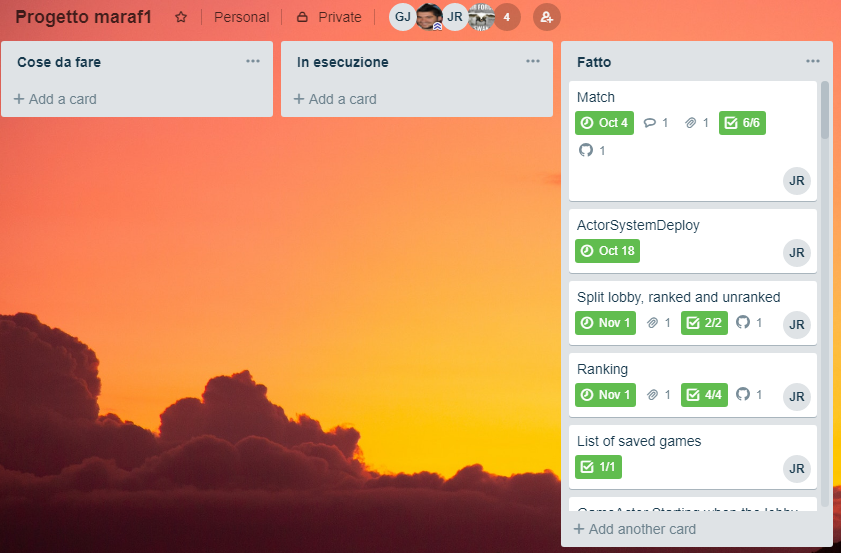
\includegraphics[width=0.8\textwidth]{trello.png}
   \caption{Screen della board di Trello a fine progetto }
\end{figure}

\end{document}
